% Copernicus Publications Manuscript Preparation Template for LaTeX Submissions
%% ---------------------------------
%% This template should be used for copernicus.cls
%% The class file and some style files are bundled in the Copernicus Latex Package which can be downloaded from the different journal webpages.
%% For further assistance please contact the Copernicus Publications at: publications@copernicus.org
%% http://publications.copernicus.org


%% Please use the following documentclass and Journal Abbreviations for Discussion Papers and Final Revised Papers.


%% 2-Column Papers and Discussion Papers
\documentclass[gmd, manuscript]{copernicus}



%% Journal Abbreviations (Please use the same for Discussion Papers and Final Revised Papers)

% Archives Animal Breeding (aab)
% Atmospheric Chemistry and Physics (acp)
% Advances in Geosciences (adgeo)
% Advances in Statistical Climatology, Meteorology and Oceanography (ascmo)
% Annales Geophysicae (angeo)
% ASTRA Proceedings (ap)
% Atmospheric Measurement Techniques (amt)
% Advances in Radio Science (ars)
% Advances in Science and Research (asr)
% Biogeosciences (bg)
% Climate of the Past (cp)
% Drinking Water Engineering and Science (dwes)
% Earth System Dynamics (esd)
% Earth Surface Dynamics (esurf)
% Earth System Science Data (essd)
% Fossil Record (fr)
% Geographica Helvetica (gh)
% Geoscientific Instrumentation, Methods and Data Systems (gi)
% Geoscientific Model Development (gmd)
% Geothermal Energy Science (gtes)
% Hydrology and Earth System Sciences (hess)
% History of Geo- and Space Sciences (hgss)
% Journal of Sensors and Sensor Systems (jsss)
% Mechanical Sciences (ms)
% Natural Hazards and Earth System Sciences (nhess)
% Nonlinear Processes in Geophysics (npg)
% Ocean Science (os)
% Proceedings of the International Association of Hydrological Sciences (piahs)
% Primate Biology (pb)
% Scientific Drilling (sd)
% SOIL (soil)
% Solid Earth (se)
% The Cryosphere (tc)
% Web Ecology (we)
% Wind Energy Science (wes)


%% \usepackage commands included in the copernicus.cls:
%\usepackage[german, english]{babel}
%\usepackage{tabularx}
%\usepackage{cancel}
%\usepackage{multirow}
%\usepackage{supertabular}
%\usepackage{algorithmic}
%\usepackage{algorithm}
%\usepackage{amsthm}
%\usepackage{float}
%\usepackage{subfig}
%\usepackage{rotating}

\usepackage{url}


\begin{document}

\title{Ellipsoids (v1.0): 3D Magnetic modelling of ellipsoidal bodies}


% \Author[affil]{given_name}{surname}

\Author[1]{Diego}{Takahashi Tomazella}
\Author[1]{Vanderlei}{C. Oliveira Jr.}

\affil[1]{Department of Geophysics, Observat\'{o}rio Nacional, Rio de Janeiro, Brazil}
%\affil[]{}

%% The [] brackets identify the author with the corresponding affiliation. 1, 2, 3, etc. should be inserted.



\runningtitle{Magnetic modelling of ellipsoids}

\runningauthor{Tomazella and Oliveira Jr.}

\correspondence{Vanderlei C. Oliveira Jr. (vandscoelho@gmail.com)}



\received{}
\pubdiscuss{} %% only important for two-stage journals
\revised{}
\accepted{}
\published{}

%% These dates will be inserted by Copernicus Publications during the typesetting process.


\firstpage{1}

\maketitle



\begin{abstract}


A considerable amount of literature has been published on the magnetic
modelling of uniformly magnetized ellipsoids since the second half of
the nineteenth century. Ellipsoids have flexibility to represent a wide
range of geometrical forms, are the only known bodies which can be
uniformly magnetized in the presence of a uniform inducing field and
are the only finite bodies for which the self-demagnetization can be treated
analytically. This property makes ellipsoids particularly useful for
modelling compact orebodies having high susceptibility. In this case,
neglecting the self-demagnetization may strongly mislead the interpretation
of these bodies by using magnetic methods. A number of previous studies
consider that the self-demagnetization can be neglected for the case in
which the geological body has an isotropic susceptibility lower than or
equal to 0.1 SI. This limiting value, however, seems to be determined
empirically and there has been no discussion about how this value was
determined. Besides, the geoscientific community lacks an easy-to-use
tool to simulate the magnetic field produced by uniformly magnetized
ellipsoids. Here, we present an integrated review of the magnetic
modelling of arbitrarily oriented triaxial, prolate and oblate
ellipsoids. Our review includes ellipsoids with both induced and
remanent magnetization, as well as with isotropic or anisotropic
susceptibility. We also discuss the ambiguity between confocal ellipsoids
with the same magnetic moment and propose a
way of determining the isotropic susceptibility above which the
self-demagnetization must be taken into consideration. Tests with
synthetic data validate our approach. Finally, we provide a set
of routines to model the magnetic field produced
by ellipsoids. The routines are written in Python language as
part of the Fatiando a Terra, which is an open-source library
for modelling and inversion in geophysics.


\end{abstract}



%\introduction  %% \introduction[modified heading if necessary]
\section{Introduction}

Based on the mathematical theory of the magnetic
induction developed by \citet{poisson1824},
\citet{maxwell1873} affirmed that, if $U$ is the
gravitational potential produced by any body
with uniform density $\rho$ and arbitrary shape at
a point $(x, y, z)$, then $-\frac{\partial U}{\partial x}$
is the magnetic scalar potential produced
at the same point by the same body
if it has a uniform magnetization oriented along $x$
with intensity $\rho$.
\citet{maxwell1873} generalized this idea as a way
of determining the magnetic scalar potential produced
by any uniformly magnetized body in a given direction.
By presuming that this uniform magnetization is due to
induction and that it is proportional to the resulting
magnetic field (intensity) inside the body, he postulated
that the resulting field must also be uniform and
parallel to the magnetization. This uniformity is due to
the fact that the resulting field is defined as the
negative gradient of the magnetic scalar potential.
As a consequence of this uniformity,
the gravitational potential $U$ at points within the
body must be a quadratic
function of the spatial coordinates.
Apparently, \citet{maxwell1873} was the first one to
postulate that ellipsoids are the only finite bodies
having a gravitational potential which satisfies this
property and hence can be uniformly magnetized
in the presence of a uniform inducing magnetic field.
This property can be extended to other bodies
defined as limiting cases of an ellipsoid
(e.g., spheres, elliptic cylinders), however all the
remaining non-ellipsoidal bodies cannot be
uniformly magnetized in the presence of a uniform
inducing field.

Another particularity of ellipsoids is that they are
the only bodies which enable an analytical computation
of its self-demagnetization.
The self-demagnetization contributes to decrease the
magnitude of the magnetization along the shortest
axes of a body.
It is a function of the body shape and gives rise
to shape anisotropy \citep{uyeda1963, thompson1986,
dunlop1997, clark1999, tauxe2003}.
It is well-established in the literature that
the self-demagnetization can be neglected if the
body has a susceptibility lower than 0.1 \unit{SI}
\citep{emerson1985, clark1986, eskola1980, guo1998,
guo2001, purss2005, hillan2013, austin2014, clark2014}.
On the other hand, neglecting the self-demagnetization in
geological bodies with high susceptibilities (> 0.1 \unit{SI})
may strongly mislead the interpretation obtained from
magnetic methods.
This limiting value, however, seems to be determined empirically
and, so far, there has been little discussion about
how it was determined.

\citet{farrar1979} demonstrated the importance of the
ellipsoidal model in taking into account the
self-demagnetization and determining reliable
drilling directions on the Tennant Creek field,
Australia.
Posteriorly, \citet{hoschke1991} also showed how the
ellipsoidal model proved to be highly successful in
locating and defining ironstone bodies in the
Tennant Creek field.
\citet{clark2000} provides a good discussion about the
influence of the self-demagnetization in magnetic
interpretation of the Osborne copper-gold deposit,
Australia. This deposit is hosted by ironstone
bodies that have very high susceptibility.
According to \citet{clark2000}, neglecting the effects
of self-demagnetisation led errors of $\approx 55^{\circ}$
in the interpreted dip.
Recently, \citet{austin2014} used magnetic modelling
and rock property measurements to show that,
contrary to previous interpretations, the magnetization
of the Candelaria iron oxide copper-gold deposit,
Chile, is not dominated by the induced component.
Rather, the deposit has a relatively weak remanent
magnetization and is strongly affected by
self-demagnetization.
These examples show the importance of the self-demagnetization
and the ellipsoidal model in
producing trustworthy geological models of
high-susceptibility orebodies, which may save significant
cost associated with drilling.

A vast literature about the magnetic
modelling of ellipsoidal bodies was developed in which
are to be found the names of many researchers.
Nevertheless, interest in this subject has not yet died
out, as is evidenced by a list of modern papers in this
field.
Besides, the geoscientific community lacks a free easy-to-use
tool to simulate the magnetic field produced by uniformly
magnetized ellipsoids.
Such a tool could prove to be useful either for teaching
and researching geophysics.

In this work, we present a review of the vast literature
about the magnetic modelling of ellipsoidal bodies and a
theoretical discussion about the determination of the
isotropic susceptibility value above which
the self-demagnetization must be taken into consideration.
We propose an alternative way of determining this value
based on the body shape and the maximum relative error
allowed in the resultant magnetization.
This alternative approach is validated
by the results obtained with numerical simulations.
We also provide a set of routines to
model the magnetic field produced by ellipsoids.
The routines are written in Python language as part of
the Fatiando a Terra \citep{uieda2013}, which is an
open-source library for modelling and inversion in geophysics.
We attempt to use the best practices of continuous
integration, documentation, unit-testing, and version-control
for the purpose of providing a reliable and easy-to-use
code.


\section{Methodology}


\subsection{Geometrical parameters and coordinate systems}


Let $(x, y, z)$ be a point referred to a Cartesian coordinate system with axes
$x$, $y$ and $z$ pointing to, respectively, North, East and down.
For convenience, we denominate this coordinate system as
\textit{main coordinate system} (Fig. \ref{fig:orientation-angles}a).
Let us consider an ellipsoidal body with centre at the point
$(x_{c}, y_{c}, z_{c})$, orientation defined by the angles
\textit{strike} $\varepsilon$, \textit{dip} $\zeta$, and \textit{rake} $\eta$
(Fig. \ref{fig:orientation-angles}a), and semi-axes defined by
positive constants $a$, $b$, $c$ (Fig. \ref{fig:orientation-angles}b).
The orientation angles \textit{strike}, \textit{dip}, and \textit{rake}
are commonly used to define the orientation of lines in structural geology
\citep{pollard2005, allmendinger2012}.
The points $(x, y, z)$ located on the surface of this ellipsoidal body
satisfy the following equation:
\begin{equation}
(\mathbf{r} - \mathbf{r}_c)^T \mathbf{A} (\mathbf{r} - \mathbf{r}_c) = 1 \: ,
\label{eq:ellipsoid_surface}
\end{equation}
where $\mathbf{r} = [\begin{array}{ccc} x & y & z \end{array} ]^{\top}$,
$\mathbf{r}_{c} = [\begin{array}{ccc} x_{c} & y_{c} & z_{c} \end{array} ]^{\top}$,
$\mathbf{A}$ is a positive definite matrix given by
\begin{equation}
\mathbf{A} = \mathbf{V}
\left[ \begin{array}{ccc}
a^{-2} & 0 & 0 \\
0 & b^{-2} & 0 \\
0 & 0 & c^{-2}
\end{array} \right] \mathbf{V}^{\top} \: ,
\label{eq:A}
\end{equation}
and $\mathbf{V}$ is an orthogonal matrix whose first, second and third columns
are defined by unit vectors $\mathbf{v}_{1}$, $\mathbf{v}_{2}$, and $\mathbf{v}_{3}$
(Fig. \ref{fig:orientation-angles}b), respectively.
The matrix $\mathbf{V}$ can be defined in terms of three rotation matrices:
\begin{equation}
\mathbf{R}_{1}(\theta) = \left[ \begin{array}{ccc}
1 & 0 & 0 \\
0 & \cos \theta & \sin \theta \\
0 & -\sin \theta & \cos \theta
\end{array} \right] \: ,
\label{eq:R1}
\end{equation}
\begin{equation}
\mathbf{R}_{2}(\theta) = \left[ \begin{array}{ccc}
\cos \theta & 0 & -\sin \theta \\
0 & 1 & 0 \\
\sin \theta & 0 & \cos \theta
\end{array} \right]
\label{eq:R2}
\end{equation}
and
\begin{equation}
\mathbf{R}_{3}(\theta) = \left[ \begin{array}{ccc}
\cos \theta & \sin \theta & 0 \\
-\sin \theta & \cos \theta & 0 \\
0 & 0 & 1
\end{array} \right] \: .
\label{eq:R3}
\end{equation}
For triaxial ellipsoids (i.e., $a > b > c$) and prolate ellipsoids
(i.e., $a > b = c$), we define the orthogonal matrix $\mathbf{V}$
as follows:
\begin{equation}
\mathbf{V} =
\mathbf{R}_{1} \left( \frac{\pi}{2} \right) \;
\mathbf{R}_{2} \left( \varepsilon \right) \;
\mathbf{R}_{1} \left( \frac{\pi}{2} - \zeta \right) \;
\mathbf{R}_{3} \left( \eta \right) \: .
\label{eq:V_triaxial_prolate}
\end{equation}
For oblate ellipsoids (i.e., $a < b = c$), we define $\mathbf{V}$ as follows:
\begin{equation}
\mathbf{V} =
\mathbf{R}_{3} \left( -\frac{\pi}{2} \right) \;
\mathbf{R}_{1} \left( \pi \right) \,
\mathbf{R}_{3} \left( \varepsilon \right) \,
\mathbf{R}_{2} \left( \frac{\pi}{2} - \zeta \right) \,
\mathbf{R}_{1} \left( \eta \right) \: .
\label{eq:V_oblate}
\end{equation}
The orthogonal matrices $\mathbf{V}$ used here for triaxial, prolate and oblate
ellipsoids (Eqs. \ref{eq:V_triaxial_prolate} and \ref{eq:V_oblate}) are
different from that used by \citet{emerson1985} and \citet{clark1986}.

The magnetic modelling of an ellipsoidal body is commonly performed
in a particular Cartesian coordinate system that is aligned
with the body semi-axes
and has the origin coincident with the body centre
(Fig. \ref{fig:orientation-angles}b).
For convenience, we denominate this particular coordinate
system as \textit{local coordinate system}.
The relationship between the Cartesian coordinates
$(\tilde{x}, \tilde{y}, \tilde{z})$ of a point in
a local coordinate system and the Cartesian
coordinates $(x, y, z)$ of the same point in the main
system is given by:
\begin{equation}
\tilde{\mathbf{r}} = \mathbf{V}^{\top} \left( \mathbf{r} - \mathbf{r}_{c} \right) \: ,
\label{eq:coord_transformation}
\end{equation}
where
$\tilde{\mathbf{r}} = [\begin{array}{ccc} \tilde{x} &
                                          \tilde{y} &
                                          \tilde{z} \end{array} ]^{\top}$,
$\mathbf{r}$ and $\mathbf{r}_{c}$
are defined in Eq. \ref{eq:ellipsoid_surface} and the matrix $\mathbf{V}$
(Eq. \ref{eq:A}) is defined according to the ellipsoid type.
Subsequently, quantities referred to the local coordinate system
(Fig. \ref{fig:orientation-angles}b) are represented with
the simbol "$\sim$".


\subsection{Theoretical background}


Consider a magnetized ellipsoid immersed in
a uniform inducing magnetic field $\mathbf{H}_{0}$ (in $\unit{Am^{-1}}$)
given by
\begin{equation}
\mathbf{H}_{0} = \| \mathbf{H}_{0} \| \left[
\begin{array}{c}
\cos I \: \cos D \\
\cos I \: \sin D \\
\sin I
\end{array}
\right] \: ,
\label{eq:H0}
\end{equation}
where $\| \cdot \|$ denotes the Euclidean norm (or 2-norm) and
$D$ and $I$ are respectively, the declination and inclination of the
local-geomagnetic field in the main coordinate system
(Fig. \ref{fig:orientation-angles}a).
This field represents the main component of the
Earth's magnetic field, which is usually assumed to be generated
by the Earth's liquid core.
In the absence of conduction currents,
the total magnetic field $\mathbf{H}(\mathbf{r})$
at the position $\mathbf{r}$ (Eq. \ref{eq:ellipsoid_surface})
of a point referred to the main
coordinate system is defined as follows \citep{sharma1966,
eskola1980, reitz1992, sttraton2007}:
\begin{equation}
\mathbf{H}(\mathbf{r}) = \mathbf{H}_{0} - \nabla V(\mathbf{r}) \: ,
\label{eq:H}
\end{equation}
where the second term is the negative gradient of
the magnetic scalar potential $V(\mathbf{r})$ given by:
\begin{equation}
V(\mathbf{r}) = -\frac{1}{4\pi} \iiint_{\vartheta}
\mathbf{M}(\mathbf{r}^{\prime})^{\top}
\nabla \left(
\frac{1}{\| \mathbf{r} - \mathbf{r}^{\prime} \|}
\right) \, dx^{\prime}dy^{\prime}dz^{\prime} \: .
\label{eq:V-potential}
\end{equation}
In this equation, $\mathbf{r}^{\prime} = [\begin{array}{ccc}
x^{\prime} & y^{\prime} & z^{\prime} \end{array} ]^{\top}$
is the position vector of a point located within the volume $\vartheta$,
the integral is conducted over the variables
$x^{\prime}$, $y^{\prime}$ and, $z^{\prime}$ and
$\mathbf{M}(\mathbf{r}^{\prime})$ is the magnetization vector
(in \unit{Am^{-1}}).
Eq. \ref{eq:V-potential} is valid anywhere,
independently if the position vector $\mathbf{r}$ represents
a point located inside or outside the magnetized body
\citep{dubois1896, reitz1992, sttraton2007}.

Based on \citeauthor{maxwell1873}'s postulate, let us
assume that the body has a uniform magnetization given by
\begin{equation}
\mathbf{M} = \mathbf{K} \, \mathbf{H}^{\dagger} \: ,
\label{eq:M-KH}
\end{equation}
where $\mathbf{H}^{\dagger}$ is the resultant uniform magnetic field
at any point within the body and $\mathbf{K}$ is a
constant and symmetrical 2nd-order tensor representing the
magnetic susceptibility of the body.
This is a good approximation for bodies at room temperature,
subjected to an inducing field $\mathbf{H}_{0}$ with
strength $\leq 10^{-3} \mu_{0}^{-1}$ \unit{A \, m^{-1}} \citep{rochette1992},
where $\mu_{0}$ represents the magnetic constant (in \unit{H \, m^{-1}}).
In this case, the susceptibility tensor $\mathbf{K}$ is commonly
represented, in the main coordinate system (Fig. \ref{fig:orientation-angles}a),
as follows:
\begin{equation}
\mathbf{K} = \mathbf{U}
\left[ \begin{array}{ccc}
k_{1} & 0 & 0 \\
0 & k_{2} & 0 \\
0 & 0 & k_{3}
\end{array} \right] \mathbf{U}^{\top} \: ,
\label{eq:K}
\end{equation}
where $k_{1} > k_{2} > k_{3}$ are the
\textit{principal susceptibilities} and $\mathbf{U}$ is
an orthogonal matrix whose columns $\mathbf{u}_{i}$,
$i = 1, 2, 3$, are unit vectors called
\textit{principal directions}.
Similarly to the matrix $\mathbf{V}$ (Eqs. \ref{eq:ellipsoid_surface},
\ref{eq:V_triaxial_prolate} and \ref{eq:V_oblate}), we define
the matrix $\mathbf{U}$ as a function
of given orientation angles $\varepsilon$, $\zeta$,
and $\eta$ depending on the ellipsoid type. For triaxial
and prolate ellipsoids, we define $\mathbf{U}$ by
using Eq. \ref{eq:V_triaxial_prolate}, whereas for oblate ellipsoids
we use Eq. \ref{eq:V_oblate}.
Notice that the orientation angles $\varepsilon$, $\zeta$,
and $\eta$ defining the orthogonal matrix $\mathbf{U}$
may be different from that angles $\varepsilon$, $\zeta$,
and $\eta$ defining the ellipsoid orientation
(Fig. \ref{fig:orientation-angles}).

If the principal susceptibilities are different from
each other, we say that the body has an
anisotropy of magnetic susceptibility (AMS).
The AMS is generally associated to the preferred orientation
of the grains of magnetic minerals forming the rock
\citep{fuller1963, uyeda1963, janak1972, hrouda1982,
thompson1986, macdonald1987, rochette1992, dunlop1997,
tauxe2003}.
For the particular case in which the principal directions
coincide with the ellipsoid axes, the matrix $\mathbf{U}$ is
equal to the matrix $\mathbf{V}$ (Eq. \ref{eq:A}).
Another important particular case is that in which the
susceptibility is isotropic and, consequently, the principal
susceptibilities $k_{1}$, $k_{2}$, and $k_{3}$ (Eq. \ref{eq:K})
are equal to a constant $\chi$. In this case, the susceptibility
tensor $\mathbf{K}$ (Eq. \ref{eq:K}) assumes the particular form
\begin{equation}
\mathbf{K} = \chi \, \mathbf{I} \: ,
\label{eq:K-isotropic}
\end{equation}
where $\mathbf{I}$ represents the identity matrix.

By using the magnetization $\mathbf{M}$ defined by Eq. \ref{eq:M-KH},
the total magnetic field $\mathbf{H}(\mathbf{r})$ (Eq. \ref{eq:H})
can be rewritten as follows:
\begin{equation}
\mathbf{H}(\mathbf{r}) = \mathbf{H}_{0}
+ \mathbf{N}(\mathbf{r}) \, \mathbf{K} \, \mathbf{H}^{\dagger} \: ,
\label{eq:H-M-uniform}
\end{equation}
where $\mathbf{N}(\mathbf{r})$ is a symmetrical matrix whose
$ij$-element $n_{ij}(\mathbf{r})$ is given by
\begin{equation}
n_{ij}(\mathbf{r}) =
\frac{1}{4\pi} \frac{\partial^{2} \, f(\mathbf{r})}
{\partial r_{i} \, \partial r_{j}}
\: , \quad i = 1, 2, 3 \: ,
\quad j = 1, 2, 3 \: ,
\label{eq:nij}
\end{equation}
$r_{1} = x$, $r_{2} = y$, $r_{3} = z$ are the elements of
the position vector $\mathbf{r}$ (Eq. \ref{eq:ellipsoid_surface}),
and
\begin{equation}
f(\mathbf{r}) = \iiint_{\vartheta}
\frac{1}{\| \mathbf{r} - \mathbf{r}^{\prime} \|}
\, dx^{\prime}dy^{\prime}dz^{\prime} \: .
\label{eq:f}
\end{equation}
Notice that the scalar function $f(\mathbf{r})$
(Eq. \ref{eq:f}) is proportional
to the gravitational potential that would be produced by the
ellipsoidal body with volume $\vartheta$ if it had a uniform density
equal to the inverse of the gravitational constant.
It can be shown that the elements $n_{ij}(\mathbf{r})$ are
finite whether $\mathbf{r}$ is a point within or without
the volume $\vartheta$ \citep{peirce1902, webster1904}.
The matrix $\mathbf{N}(\mathbf{r})$ (Eq. \ref{eq:H-M-uniform})
is called \textit{depolarization tensor} \citep{soliverez1981, soliverez2008, soliverez2016}.

The following part of this paper moves on to describe
the magnetic field $\mathbf{H}(\mathbf{r})$
(Eq. \ref{eq:H-M-uniform}) at points located
both within and without the volume $\vartheta$ of the ellipsoidal
body. However, the mathematical developments are conveniently
performed in the local coordinate system (Fig. \ref{fig:orientation-angles}b)
related to the respective ellipsoidal body.

\subsection{Coordinate transformation}

To continue our description of the magnetic modelling of
ellipsoidal bodies, it is convenient to perform two
important coordinate transformations.
The first one transforms the scalar function
$f(\mathbf{r})$ (Eq. \ref{eq:f}) from the
main coordinate system (Fig. \ref{fig:orientation-angles}a)
into a new scalar function
$\tilde{f}(\tilde{\mathbf{r}})$ referred to the
local coordinate system (Fig. \ref{fig:orientation-angles}b).
The function $\tilde{f}(\tilde{\mathbf{r}})$ was first
presented by \citet{dirichlet1839} to describe the gravitational potential
produced by homogeneous ellipsoids.
Posteriorly, several authors also deduced and used this function
for describing the magnetic and gravitational fields produced
by triaxial, prolate, and oblate ellipsoids
\citep{maxwell1873, thomson1879, dubois1896,
peirce1902, webster1904, kellogg1929, stoner1945, osborn1945,
peake1953, macmillan1958, chang1961, lowes1974,  clark1986,
tejedor1995, sttraton2007}.

It is convenient to use $\tilde{f}^{\dagger}(\tilde{\mathbf{r}})$
and $\tilde{f}^{\ddagger}(\tilde{\mathbf{r}})$ to define
the function $\tilde{f}(\tilde{\mathbf{r}})$ evaluated,
respectively, at points
$\tilde{\mathbf{r}}$ inside and outside the volume $\vartheta$ of the
ellipsoidal body.
The scalar function $\tilde{f}^{\dagger}(\tilde{\mathbf{r}})$
is given by
\begin{equation}
\tilde{f}^{\dagger}(\tilde{\mathbf{r}}) = \pi \, abc \,
\int_{0}^{\infty} \left( 1
- \frac{\tilde{x}^{2}}{a^{2} + u}
- \frac{\tilde{y}^{2}}{b^{2} + u}
- \frac{\tilde{z}^{2}}{c^{2} + u} \right)
\frac{1}{R(u)} \, du \: , \quad \tilde{\mathbf{r}} \in \vartheta \: ,
\label{eq:fi-tilde}
\end{equation}
where
\begin{equation}
R(u) = \sqrt{\left( a^{2} + u \right)\left( b^{2} + u \right)\left( c^{2} + u \right)} \: .
\label{eq:R}
\end{equation}
This function represents the gravitational potential
that would be produced by the ellipsoidal body at
points located within its volume $\vartheta$ if it
had a uniform density equal to the inverse of the
gravitational constant.
Notice that, in this case, the gravitational potential
is a quadratic function of the spatial coordinates
$\tilde{x}$, $\tilde{y}$, and $\tilde{z}$, which
supported \citeauthor{maxwell1873}'s (\citeyear{maxwell1873})
postulate about uniformly magnetized ellipsoids.
In a similar way, the function $\tilde{f}^{\ddagger}(\tilde{\mathbf{r}})$
is given by
\begin{equation}
\tilde{f}^{\ddagger}(\tilde{\mathbf{r}}) = \pi \, abc \,
\int_{\lambda}^{\infty} \left( 1
- \frac{\tilde{x}^{2}}{a^{2} + u}
- \frac{\tilde{y}^{2}}{b^{2} + u}
- \frac{\tilde{z}^{2}}{c^{2} + u} \right)
\frac{1}{R(u)} \, du \: , \quad \tilde{\mathbf{r}} \not\in \vartheta \: ,
\label{eq:fe-tilde}
\end{equation}
where $R(u)$ is defined by Eq. \ref{eq:R} and the
parameter $\lambda$ is defined according to the
ellipsoid type as a function of the spatial coordinates
 $\tilde{x}$, $\tilde{y}$, and $\tilde{z}$ (see Appendix B).
For readers interested in additional information about the
parameter $\lambda$, we recommend \citet[p.~234]{webster1904},
\citet[p.~184]{kellogg1929} and \citet{clark1986}.

The second important coordinate transformation is defined
with respect to Eq. \ref{eq:H-M-uniform}.
By properly using the orthogonality of matrix $\mathbf{V}$
(Eq. \ref{eq:A}),
the magnetic field $\mathbf{H}(\mathbf{r})$
(Eq. \ref{eq:H-M-uniform}) can be transformed
from the main coordinate system (Fig. \ref{fig:orientation-angles}a)
to the local coordinate system (Fig. \ref{fig:orientation-angles}b) as follows:
\begin{equation}
\underbrace{\mathbf{V}^{\top} \mathbf{H}(\mathbf{r})}_{\tilde{\mathbf{H}}(\tilde{\mathbf{r}})} =
\underbrace{\mathbf{V}^{\top} \mathbf{H}_{0}}_{\tilde{\mathbf{H}}_{0}}
+ \underbrace{\mathbf{V}^{\top} \mathbf{N}(\mathbf{r}) \mathbf{V}}
_{\tilde{\mathbf{N}}(\tilde{\mathbf{r}})} \;
\underbrace{\mathbf{V}^{\top} \mathbf{K} \mathbf{V}}
_{\tilde{\mathbf{K}}} \;
\underbrace{\mathbf{V}^{\top} \mathbf{H}^{\dagger}}
_{\tilde{\mathbf{H}}^{\dagger}} \: ,
\label{eq:H-tilde}
\end{equation}
where the superscript "$\sim$" denotes quantities
referred to the respective local coordinate system.

In Eq. \ref{eq:H-tilde}, the transformed
depolarization tensor $\tilde{\mathbf{N}}(\tilde{\mathbf{r}})$
is calculated as a function of the original depolarization
tensor $\mathbf{N}(\mathbf{r})$ (Eq. \ref{eq:H-M-uniform}).
In this case, the elements of $\tilde{\mathbf{N}}(\tilde{\mathbf{r}})$
are calculated as a function of the second derivatives of the
function $f(\mathbf{r})$ (Eq. \ref{eq:f}),
which is defined in the main coordinate system (Fig. \ref{fig:orientation-angles}a).
It can be shown (Appendix A), however, that the
elements $\tilde{n}_{ij}(\tilde{\mathbf{r}})$ of
$\tilde{\mathbf{N}}(\tilde{\mathbf{r}})$ can also be calculated
as follows:
\begin{equation}
\tilde{n}_{ij}(\tilde{\mathbf{r}}) =
\frac{1}{4\pi} \frac{\partial^{2} \, \tilde{f}(\tilde{\mathbf{r}})}
{\partial \tilde{r}_{i} \, \partial \tilde{r}_{j}}
\: , \quad i = 1, 2, 3 \: , \quad j = 1, 2, 3 \: ,
\label{eq:nij-tilde}
\end{equation}
where $\tilde{r}_{1} = \tilde{x}$, $\tilde{r}_{2} = \tilde{y}$,
and $\tilde{r}_{3} = \tilde{z}$ are the elements of the
transformed vector $\tilde{\mathbf{r}}$ (Eq. \ref{eq:coord_transformation})
and $\tilde{f}(\tilde{\mathbf{r}})$ is given by Eq. \ref{eq:fi-tilde}
or \ref{eq:fe-tilde}, depending if $\tilde{\mathbf{r}}$ represents a
point located within or without the volume $\vartheta$ of the
ellipsoidal body.


\subsection{Transformed depolarization tensors $\tilde{\mathbf{N}}(\tilde{\mathbf{r}})$}


\subsubsection{Depolarization tensor $\tilde{\mathbf{N}}^{\dagger}$}


Let $\tilde{\mathbf{N}}^{\dagger}$ be the transformed
depolarization tensor calculated for the case in which
$\tilde{\mathbf{r}}$ (Eq. \ref{eq:coord_transformation})
represents a point located inside
the ellipsoidal body. In this case,
the elements of $\tilde{\mathbf{N}}^{\dagger}$
are calculated according to Eq. \ref{eq:nij-tilde},
with $\tilde{f}(\tilde{\mathbf{r}})$ given by
$\tilde{f}^{\dagger}(\tilde{\mathbf{r}})$ (Eq. \ref{eq:fi-tilde}).
As we have already pointed out, the
$\tilde{f}^{\dagger}(\tilde{\mathbf{r}})$ (Eq. \ref{eq:fi-tilde}) is a
quadratic function of the spatial coordinates $\tilde{x}$,
$\tilde{y}$ and $\tilde{z}$. Consequently, the
elements $\tilde{n}^{\dagger}_{ij}$, $i = 1, 2, 3$,
$j = 1, 2, 3$, of $\tilde{\mathbf{N}}^{\dagger}$
do not depend on the elements of the transformed position
vector $\tilde{\mathbf{r}}$ (Eq. \ref{eq:coord_transformation}).
Besides, the off-diagonal elements are zero and
the diagonal elements are given by \citep{stoner1945}:
\begin{equation}
\tilde{n}^{\dagger}_{ii} = \frac{abc}{2}
\int_{0}^{\infty} \frac{1}{\left( e_{i}^{2}
+ u \right) R(u)} \, du \: , \quad i = 1, 2, 3 \: ,
\label{eq:n-tilde-dagger-ii}
\end{equation}
where $R(u)$ is defined by Eq. \ref{eq:R} and
$e_{1} = a$, $e_{2} = b$, and $e_{3} = c$. These elements
are commonly known as \textit{demagnetizing factors}
and are defined according to the ellipsoid type.
Here, we calculate the demagnetizing factors in the \unit{SI}
system. Consequently, they satisfies the condition
$\tilde{n}^{\dagger}_{11} + \tilde{n}^{\dagger}_{22} +
\tilde{n}^{\dagger}_{33} = 1$, independently of the
ellipsoid type.
It is worth stressing that, according to Eq. \ref{eq:n-tilde-dagger-ii},
the demagnetizing factors $\tilde{n}^{\dagger}_{ii}$ are
constants defined by the ellipsoid semi-axes $a$, $b$, and $c$.

Notice that, according to Eqs. \ref{eq:H-tilde}
and \ref{eq:N-tilde-VT-N-V},
\begin{equation}
\mathbf{N}(\mathbf{r}) =
\mathbf{V} \, \tilde{\mathbf{N}}^{\dagger} \,
\mathbf{V}^{\top} \: ,
\label{eq:N-V-N-dagger-VT}
\end{equation}
where $\tilde{\mathbf{N}}^{\dagger}$ is a diagonal
matrix and $\mathbf{V}$ (Eq. \ref{eq:A}) is an orthogonal matrix.
This equation shows that, for the particular case
in which $\mathbf{r}$ and consequently $\tilde{\mathbf{r}}$
represent a point inside the
volume $\vartheta$ of the ellipsoid, the elements
$\tilde{n}^{\dagger}_{ii}$
of $\tilde{\mathbf{N}}^{\dagger}$ represent the eigenvalues while the
columns of $\mathbf{V}$ represent the eigenvectors of the
original depolarization tensor $\mathbf{N}(\mathbf{r})$.


\subparagraph*{Triaxial ellipsoids}


For triaxial ellipsoids (e.g., $a > b > c$), the demagnetizing
factors obtained by solving Eq. \ref{eq:n-tilde-dagger-ii}
are given by:
\begin{equation}
\tilde{n}^{\dagger}_{11} = \frac{abc}
{\left( a^{2} - c^{2} \right)^{\frac{1}{2}}
\left( a^{2} - b^{2} \right)}
\left[ F(\kappa, \phi) - E(\kappa, \phi) \right] \: ,
\label{eq:n-tilde-dagger-11-triaxial}
\end{equation}
\begin{equation}
\tilde{n}^{\dagger}_{22} =
-\frac{abc}
{\left( a^{2} - c^{2} \right)^{\frac{1}{2}}
\left( a^{2} - b^{2} \right)}
\left[ F(\kappa, \phi) - E(\kappa, \phi) \right] +
\frac{abc}
{\left( a^{2} - c^{2} \right)^{\frac{1}{2}}
\left( b^{2} - c^{2} \right)} E(\kappa, \phi)
- \frac{c^{2}}{b^{2} - c^{2}}
\label{eq:n-tilde-dagger-22-triaxial}
\end{equation}
and
\begin{equation}
\tilde{n}^{\dagger}_{33} =
-\frac{abc}
{\left( a^{2} - c^{2} \right)^{\frac{1}{2}}
\left( b^{2} - c^{2} \right)} E(\kappa, \phi) +
\frac{b^{2}}{b^{2} - c^{2}} \: ,
\label{eq:n-tilde-dagger-33-triaxial}
\end{equation}
where
\begin{equation}
F(\kappa, \phi) =
\int^{\phi}_{0}
\frac{1}{\left( 1 - \kappa^{2} \sin^{2} \psi \right)^{\frac{1}{2}}}
d\psi \: ,
\label{eq:F-kappa-phi}
\end{equation}
and
\begin{equation}
E(\kappa, \phi) =
\int^{\phi}_{0}
\left( 1 - \kappa^{2} \sin^{2} \psi \right)^{\frac{1}{2}}
d\psi \: ,
\label{eq:E-kappa-phi}
\end{equation}
with $\kappa = \left[ \left( a^{2} - b^{2} \right) /
\left( a^{2} - c^{2} \right) \right]^{\frac{1}{2}}$ and
$\cos \phi = c/a$.
The functions $F(\kappa, \phi)$ (Eq. \ref{eq:F-kappa-phi}) and
$E(\kappa, \phi)$ (Eq. \ref{eq:E-kappa-phi}) are
called Legendre's normal elliptic integrals of the first and
second kind, respectivelly. \citet{stoner1945} presented a
detailed deduction of the demagnetizing factors $\tilde{n}^{\dagger}_{11}$
(Eq. \ref{eq:n-tilde-dagger-11-triaxial}), $\tilde{n}^{\dagger}_{22}$
(Eq. \ref{eq:n-tilde-dagger-22-triaxial}) and $\tilde{n}^{\dagger}_{33}$
(Eq. \ref{eq:n-tilde-dagger-33-triaxial}). \citet{clark1986} presented similar
formulas. It can be shown that these demagnetizing factors
satisfy the conditions
$\tilde{n}^{\dagger}_{11} + \tilde{n}^{\dagger}_{22} + \tilde{n}^{\dagger}_{33} = 1$
and
$\tilde{n}^{\dagger}_{11} < \tilde{n}^{\dagger}_{22} < \tilde{n}^{\dagger}_{33}$.


\subparagraph*{Prolate ellipsoids}


For prolate ellipsoids (e.g., $a > b = c$), the demagnetizing
factors obtained by solving Eq. \ref{eq:n-tilde-dagger-ii}
are given by:
\begin{equation}
\tilde{n}^{\dagger}_{11} = \frac{1}{m^{2} - 1}
\left\lbrace \frac{m}{\left( m^{2} - 1 \right)^{\frac{1}{2}}}
\ln \left[ m + \left( m^{2} - 1 \right)^{\frac{1}{2}} \right]
- 1 \right\rbrace
\label{eq:n-tilde-dagger-11-prolate}
\end{equation}
and
\begin{equation}
\tilde{n}^{\dagger}_{22} = \frac{1}{2} \left(1 - \tilde{n}^{\dagger}_{11} \right) \: ,
\label{eq:n-tilde-dagger-22-prolate}
\end{equation}
where $\tilde{n}^{\dagger}_{33} = \tilde{n}^{\dagger}_{22}$,
with $\tilde{n}^{\dagger}_{11}$ defined in
Eq. \ref{eq:n-tilde-dagger-11-prolate} and $m = a/b$.
The detailed deduction of the demagnetizing factors
$\tilde{n}^{\dagger}_{11}$ (Eq. \ref{eq:n-tilde-dagger-11-prolate})
and $\tilde{n}^{\dagger}_{22}$ (Eq. \ref{eq:n-tilde-dagger-22-prolate})
can be found, for example, in \citet{stoner1945}.
These formulas were posteriorly presented by \citet{emerson1985}.
It can be shown that these demagnetizing factors
satisfy the conditions
$\tilde{n}^{\dagger}_{11} + 2 \; \tilde{n}^{\dagger}_{22} = 1$
and
$\tilde{n}^{\dagger}_{11} < \tilde{n}^{\dagger}_{22}$.


\subparagraph*{Oblate ellipsoids}


For oblate ellipsoids (e.g., $a < b = c$), the demagnetizing
factors obtained by solving Eq. \ref{eq:n-tilde-dagger-ii}
are given by:
\begin{equation}
\tilde{n}^{\dagger}_{11} =
\frac{1}{1 - m^{2}} \left[
1 - \frac{m}{\left( 1 - m^{2} \right)^{\frac{1}{2}}} \cos^{-1}m
\right]
\label{eq:n-tilde-dagger-11-oblate}
\end{equation}
and
\begin{equation}
\tilde{n}^{\dagger}_{22} = \frac{1}{2} \left(1 - \tilde{n}^{\dagger}_{11} \right) \: ,
\label{eq:n-tilde-dagger-22-oblate}
\end{equation}
where $\tilde{n}^{\dagger}_{33} = \tilde{n}^{\dagger}_{22}$,
with $\tilde{n}^{\dagger}_{11}$ defined in
Eq. \ref{eq:n-tilde-dagger-11-oblate} and $m = a/b$.
The detailed deduction of these demagnetizing factors
can be found, for example, in \citet{stoner1945}.
These formulas can also be found in \citet{emerson1985}.
The only difference, however, is that \citet{emerson1985} replaced
the term $\cos^{-1}$ by a term $\tan^{-1}$, according to
the trigonometric identity
$\tan^{-1}x = \cos^{-1}(1/\sqrt{x^{2} + 1})$, $x > 0$.
It can be shown that these demagnetizing factors
satisfy the conditions
$\tilde{n}^{\dagger}_{11} + 2 \; \tilde{n}^{\dagger}_{22} = 1$
and
$\tilde{n}^{\dagger}_{11} > \tilde{n}^{\dagger}_{22}$.


\subsubsection{Depolarization tensor $\tilde{\mathbf{N}}^{\ddagger}(\tilde{\mathbf{r}})$}


The elements $\tilde{n}^{\ddagger}_{ij}(\tilde{\mathbf{r}})$,
$i = 1, 2, 3$, $j = 1, 2, 3$, of the transformed depolarization tensor
$\tilde{\mathbf{N}}^{\ddagger}(\tilde{\mathbf{r}})$
are calculated according to Eq. \ref{eq:nij-tilde}, with
$\tilde{f}(\tilde{\mathbf{r}})$ given by $\tilde{f}^{\ddagger}(\tilde{\mathbf{r}})$
(Eq. \ref{eq:fe-tilde}).
By following \citet{clark1986}, the diagonal elements
$\tilde{n}^{\ddagger}_{ii}(\tilde{\mathbf{r}})$
and the off-diagonal elements
$\tilde{n}^{\ddagger}_{ij}(\tilde{\mathbf{r}})$, $i = 1, 2, 3$,
$j = 1, 2, 3$, are given by
\begin{equation}
\tilde{n}^{\ddagger}_{ii}(\tilde{\mathbf{r}}) =
-\frac{abc}{2}
\left( \frac{\partial \lambda}{\partial \tilde{r}_{i}} \, h_{i} \, \tilde{r}_{i}
+ g_{i} \right)
\label{eq:n-tilde-ddagger-ii}
\end{equation}
and
\begin{equation}
\tilde{n}^{\ddagger}_{ij}(\tilde{\mathbf{r}}) =
-\frac{abc}{2} \left(
\frac{\partial \lambda}{\partial \tilde{r}_{i}} \, h_{j} \, \tilde{r}_{j}
\right) \: ,
\label{eq:n-tilde-ddagger-ij}
\end{equation}
where
\begin{equation}
h_{i} = -\frac{1}{\left( e_{i}^{2} + \lambda \right) R(\lambda)} \: ,
\label{eq:hi}
\end{equation}
\begin{equation}
g_{i} = \int_{\lambda}^{\infty} \frac{1}{\left( e_{i}^{2} + u \right) R(u)} du \: ,
\label{eq:gi}
\end{equation}
$e_{1} = a$, $e_{2} = b$, $e_{3} = c$, and
$\frac{\partial \lambda}{\partial \tilde{r}_{i}}$
is defined in Appendix B (Eq. \ref{eq:dlambda}).
The functions $g_{i}$ (Eq. \ref{eq:gi}) are defined according
to the ellipsoid type.
Notice that the elements $\tilde{n}^{\ddagger}_{ii}(\tilde{\mathbf{r}})$
(Eq. \ref{eq:n-tilde-ddagger-ii}) and
$\tilde{n}^{\ddagger}_{ij}(\tilde{\mathbf{r}})$
(Eq. \ref{eq:n-tilde-ddagger-ij})
are proportional to the second derivatives of the function
$\tilde{f}^{\ddagger}(\tilde{\mathbf{r}})$ (Eq. \ref{eq:fe-tilde}),
which is harmonic. Consequently, the diagonal elements
$\tilde{n}^{\ddagger}_{ii}(\tilde{\mathbf{r}})$ satisfy the condition
$\tilde{n}^{\ddagger}_{11}(\tilde{\mathbf{r}}) +
\tilde{n}^{\ddagger}_{22}(\tilde{\mathbf{r}}) +
\tilde{n}^{\ddagger}_{33}(\tilde{\mathbf{r}}) = 0$ for any
point $\tilde{\mathbf{r}}$ outside the ellipsoid, independently
of the ellipsoid type.


\subparagraph*{Triaxial ellipsoids}


For triaxial ellipsoids (e.g., $a > b > c$), the functions
$g_{i}$ (Eq. \ref{eq:gi}) are defined as follows:
\begin{equation}
g_{1} = \frac{2}{\left( a^{2} - b^{2} \right) \left( a^{2} - c^{2} \right)^{\frac{1}{2}}}
\left[ F(\kappa, \phi) - E(\kappa, \phi) \right] \: ,
\label{eq:g1-triaxial}
\end{equation}
%\begin{equation}
%g_{2} = \frac{2 \left( a^{2} - c^{2} \right)^{\frac{1}{2}}}
%{\left( a^{2} - b^{2} \right)\left( b^{2} - c^{2} \right)}
%\left[ E\left(\kappa, \phi \right)
%- \frac{\left( b^{2} - c^{2} \right)}{\left( a^{2} - c^{2} \right)}
%F\left(\kappa, \phi \right)
%- \frac{\kappa^{2} \sin\phi \, \cos\phi}
%{\left( 1 - \kappa^{2} \sin^{2}\phi \right)^{\frac{1}{2}}}
%\right]
%\label{eq:g2-triaxial}
%\end{equation}
\begin{equation}
g_{2} = \frac{2 \left( a^{2} - c^{2} \right)^{\frac{1}{2}}}
{\left( a^{2} - b^{2} \right)\left( b^{2} - c^{2} \right)}
\left\lbrace
E\left(\kappa, \phi \right)
- \left( \frac{b^{2} - c^{2}}{a^{2} - c^{2}} \right)
F\left(\kappa, \phi \right) -
\frac{a^{2} - b^{2}}{\left( a^{2} - c^{2} \right)^{\frac{1}{2}}} \left[
\frac{c^{2} + \lambda}{\left( a^{2} + \lambda \right)\left( b^{2} + \lambda \right)}
\right]^{\frac{1}{2}} \right\rbrace
\label{eq:g2-triaxial}
\end{equation}
and
%\begin{equation}
%g_{3} = \frac{2}{\left( b^{2} - c^{2} \right) \left( a^{2} - c^{2} \right)^{\frac{1}{2}}}
%\left[ \frac{\sin\phi \left( 1 - \kappa^{2} \sin^{2}\phi \right)^{\frac{1}{2}}}
%{\cos\phi}  - E\left(\kappa, \phi \right) \right]
%\: ,
%\label{eq:g3-triaxial}
%\end{equation}
\begin{equation}
g_{3} = \frac{2}{\left( b^{2} - c^{2} \right) \left( a^{2} - c^{2} \right)^{\frac{1}{2}}}
E\left(\kappa, \phi \right) +
\frac{2}{b^{2} - c^{2}}
\left[
\frac{b^{2} + \lambda}{\left( a^{2} + \lambda \right)\left( c^{2} + \lambda \right)}
\right]^{\frac{1}{2}}
\: ,
\label{eq:g3-triaxial}
\end{equation}
where $F(\kappa, \phi)$ and $E(\kappa, \phi)$ are defined by
Eqs. \ref{eq:E-kappa-phi} and \ref{eq:F-kappa-phi}, but with
$\sin \phi = \sqrt{\left( a^{2} - c^{2} \right)/\left( a^{2} + \lambda \right)}$.
A detailed deduction of these formulas was presented by \citet{tejedor1995}.
Similar formulas can also be found in \citet{clark1986}.


\subparagraph*{Prolate ellipsoids}


For prolate (e.g., $a > b = c$) ellipsoids, the functions
$g_{i}$ (Eq. \ref{eq:gi}) are given by:
\begin{equation}
g_{1} =  \frac{2}{\left( a^{2} - b^{2} \right)^{\frac{3}{2}}}
\left\lbrace
\ln \left[ \frac{\left( a^{2} - b^{2} \right)^{\frac{1}{2}} +
                 \left( a^{2} + \lambda \right)^{\frac{1}{2}}}{
                 \left( b^{2} + \lambda \right)^{\frac{1}{2}}} \right] -
\left( \frac{a^{2} - b^{2}}{a^{2} + \lambda} \right)^{\frac{1}{2}}
\right\rbrace
\label{eq:g1-prolate}
\end{equation}
and
\begin{equation}
g_{2} =  \frac{1}{\left( a^{2} - b^{2} \right)^{\frac{3}{2}}}
\left\lbrace
\frac{\left[ \left( a^{2} - b^{2} \right)
             \left( a^{2} + \lambda \right) \right]^{\frac{1}{2}}}
     {b^{2} + \lambda} -
\ln \left[ \frac{\left( a^{2} - b^{2} \right)^{\frac{1}{2}} +
                 \left( a^{2} + \lambda \right)^{\frac{1}{2}}}{
                 \left( b^{2} + \lambda \right)^{\frac{1}{2}}} \right]
\right\rbrace \: ,
\label{eq:g2-prolate}
\end{equation}
where $g_{3} = g_{2}$.
These formulas can be obtained by properly manipulating those
presented by \citet{emerson1985}.


\subparagraph*{Oblate ellipsoids}


For oblate (e.g., $a < b = c$) ellipsoids, the functions
$g_{i}$ (Eq. \ref{eq:gi}) are given by:
\begin{equation}
g_{1} =  \frac{2}{\left( b^{2} - a^{2} \right)^{\frac{3}{2}}}
\left\lbrace
\left( \frac{b^{2} - a^{2}}{a^{2} + \lambda}\right)^{\frac{1}{2}} -
\tan^{-1} \left[ \left( \frac{b^{2} - a^{2}}{a^{2} + \lambda}\right)^{\frac{1}{2}} \right]
\right\rbrace
\label{eq:g1-oblate}
\end{equation}
and
\begin{equation}
g_{2} =  \frac{1}{\left( b^{2} - a^{2} \right)^{\frac{3}{2}}}
\left\lbrace
\tan^{-1} \left[ \left( \frac{b^{2} - a^{2}}{a^{2} + \lambda}\right)^{\frac{1}{2}} \right] -
\frac{\left[ \left( b^{2} - a^{2} \right)
             \left( a^{2} + \lambda \right) \right]^{\frac{1}{2}}}
     {b^{2} + \lambda}
\right\rbrace \: ,
\label{eq:g2-oblate}
\end{equation}
where $g_{3} = g_{2}$.
Similarly to the case of prolate ellipsoid shown previously,
these formulas can be obtained by properly manipulating those
presented by \citet{emerson1985}.


\subsection{Internal magnetic field and magnetization}


By considering $\tilde{\mathbf{r}}$ as a point within the
volume $\vartheta$ of the ellipsoid and using the Maxwell's postulate
about the uniformity of the magnetic field $\mathbf{H}(\mathbf{r})$
inside ellipsoidal bodies, we can use Eq. \ref{eq:H-tilde}
for defining the resultant uniform magnetic field $\tilde{\mathbf{H}}^{\dagger}$
inside the ellipsoidal body as follows:
\begin{equation}
\tilde{\mathbf{H}}^{\dagger} =
\left( \mathbf{I} + \tilde{\mathbf{N}}^{\dagger} \, \tilde{\mathbf{K}} \right)^{-1}
\tilde{\mathbf{H}}_{0} \: ,
\label{eq:Hi-tilde}
\end{equation}
where $\mathbf{I}$ is the identity matrix and
$\tilde{\mathbf{N}}^{\dagger}$ is defined in the
previous section.

Let us pre-multiply the uniform internal field $\tilde{\mathbf{H}}^{\dagger}$
(Eq. \ref{eq:Hi-tilde}) by the transformed
susceptibility tensor $\tilde{\mathbf{K}}$
(Eq. \ref{eq:H-tilde}) to obtain
\begin{equation}
\begin{split}
\tilde{\mathbf{M}}
&= \tilde{\mathbf{K}}
\left( \mathbf{I} + \tilde{\mathbf{N}}^{\dagger} \, \tilde{\mathbf{K}} \right)^{-1}
\tilde{\mathbf{H}}_{0} \\
&=
\left( \mathbf{I} + \tilde{\mathbf{K}} \, \tilde{\mathbf{N}}^{\dagger} \right)^{-1}
\tilde{\mathbf{K}} \, \tilde{\mathbf{H}}_{0}
\end{split} \: ,
\label{eq:M-tilde}
\end{equation}
where $\tilde{\mathbf{M}}$
represents the transformed magnetization, as can be easily
verified by using Eqs. \ref{eq:M-KH} and \ref{eq:H-tilde}.
The matrix identity used for obtaining the second line of Eq.
\ref{eq:M-tilde} is given by \citet[p. ~151]{searle1982}.

Equation \ref{eq:M-tilde} can be easily generalized for the case in
which the ellipsoid has also a uniform remanent magnetization
$\tilde{\mathbf{M}}_{R}$. Let us first consider that
the uniform remanent magnetization satisfies the condition
$\tilde{\mathbf{H}}_{A} = \tilde{\mathbf{K}}^{-1} \tilde{\mathbf{M}}_{R}$,
where $\tilde{\mathbf{H}}_{A}$ represents a hypothetical
uniform ancient field. Then, if we assume that $\tilde{\mathbf{H}}_{0}$,
in Eqs. \ref{eq:Hi-tilde} and \ref{eq:M-tilde},
is in fact the sum of the inducing magnetic field $\tilde{\mathbf{H}}_{0}$
and the hypothetical ancient field $\tilde{\mathbf{H}}_{A}$, we obtain the
following generalized equation
\begin{equation}
\mathbf{M} = \mathbf{\Lambda}
\left(\mathbf{K} \, \mathbf{H}_{0} + \mathbf{M}_{R} \right) \: ,
\label{eq:M-remanence}
\end{equation}
where
\begin{equation}
\mathbf{\Lambda} = \mathbf{V}
\left( \mathbf{I} + \tilde{\mathbf{K}} \, \tilde{\mathbf{N}}^{\dagger} \right)^{-1}
\mathbf{V}^{\top} \: .
\label{eq:Lambda}
\end{equation}
Despite of the coordinate system transformation represented by the
matrix $\mathbf{V}$ (Eq. \ref{eq:A}),
Eq. \ref{eq:M-remanence} is consistent with that given by
\citet[Eq. ~38]{clark1986}. It shows the combined effect of the
anisotropy of magnetic susceptibility (AMS) and the shape anisotropy.
The AMS is represented by the susceptibility tensor $\mathbf{K}$
(Eq. \ref{eq:K}) and reflects the
preferred orientation of the magnetic minerals forming the
body. The susceptibility tensor appears in Eq. \ref{eq:M-remanence},
defined in the main coordinate system (Fig. \ref{fig:orientation-angles}a),
and Eq. \ref{eq:Lambda}, defined in the local coordinate system
(Fig. \ref{fig:orientation-angles}b).
The shape anisotropy is represented, in Eq. \ref{eq:M-remanence}, by the
depolarization tensor $\tilde{\mathbf{N}}^{\dagger}$ and
reflects the self-demagnetization associated to the body shape.
Notice that the resultant magnetization $\mathbf{M}$
(Eq. \ref{eq:M-remanence}) does not necessarily have
the same direction as the inducing field $\mathbf{H}_{0}$
(Eq. \ref{eq:H0}).
The angular difference between the resultant magnetization
and the inducing field depends on the combined effect of the
anisotropy of magnetic susceptibility and the shape anisotropy.

For the particular case in which the susceptibility is isotropic,
the susceptibility tensor is defined according to Eq. \ref{eq:K-isotropic}.
In this case, the magnetization $\mathbf{M}$ (Eqs. \ref{eq:M-KH} and \ref{eq:M-remanence}),
referred to the main coordinate system (Fig. \ref{fig:orientation-angles}a),
and the matrix $\mathbf{\Lambda}$ (Eq. \ref{eq:Lambda})
can be rewritten as follows:
\begin{equation}
\mathbf{M} = \mathbf{\Lambda} \left( \chi \, \mathbf{H}_{0} +
\mathbf{M}_{R} \right) \: ,
\label{eq:M-K-isotropic}
\end{equation}
and
\begin{equation}
\mathbf{\Lambda} = \mathbf{V}
\left( \mathbf{I} + \chi \, \tilde{\mathbf{N}}^{\dagger} \right)^{-1}
\mathbf{V}^{\top} \: .
\label{eq:Lambda-K-isotropic}
\end{equation}
Despite the coordinate transformation represented by
matrix $\mathbf{V}$ (Eq. \ref{eq:A}),
this equation is in perfect agreement with those presented
by \citet[Eqs. ~13--15]{guo2001}.
The first term, depending on the inducing field $\mathbf{H}_{0}$
(Eq. \ref{eq:H0}),
represents the induced magnetization whereas the term depending on
$\mathbf{M}_{R}$ is the remanent magnetization.
Equation \ref{eq:M-K-isotropic} reveals that, as pointed out by
many authors
\citep[e.g.,][]{maxwell1873, dubois1896, stoner1945, clark1986, sttraton2007},
the induced magnetization opposes the inducing field
if it is parallel to an ellipsoid axis,
independently of the ellipsoid type. Otherwise, the
magnetization is not necessarily parallel to
the inducing field.
If we additionally consider that $\chi << 1$, the matrix
$\mathbf{\Lambda}$ (Eq. \ref{eq:Lambda-K-isotropic})
approaches to the identity and the magnetization
$\mathbf{M}$ (Eq. \ref{eq:M-K-isotropic})
can be approximated by:
\begin{equation}
\breve{\mathbf{M}} = \chi \, \mathbf{H}_{0} +
\mathbf{M}_{R} \: ,
\label{eq:M-approx}
\end{equation}
which is the classical equation describing the resultant
magnetization in applied geophysics \citep[p. ~89]{blakely1996}.
Notice that, in this particular case, the induced magnetization
is parallel to the inducing field $\mathbf{H}_{0}$ (Eq. \ref{eq:H0}),
whether it is parallel to an ellipsoid axis or not.
Usually, Eq. \ref{eq:M-approx}
is considered a good approximation for $\chi \leq 0.1$ \unit{SI}.
Although this value has been largely used in the literature,
there have been few empirical and/or theoretical investigations
about it.


\subsubsection{Relationship between $\chi$ and the relative error in $\breve{\mathbf{M}}$}


In the case of isotropic susceptibility, the resultant magnetization
$\mathbf{M}$ (Eq. \ref{eq:M-K-isotropic}) may be determined by solving the
following linear system:
\begin{equation}
\mathbf{\Lambda}^{-1} \, \mathbf{M} = \chi \, \mathbf{H}_{0} +
\mathbf{M}_{R} \: ,
\label{eq:M-K-isotropic-inverse-Lambda}
\end{equation}
where, according to Eq. \ref{eq:Lambda-K-isotropic},
\begin{equation}
\mathbf{\Lambda}^{-1} = \mathbf{V}
\left( \mathbf{I} + \chi \, \tilde{\mathbf{N}}^{\dagger} \right)
\mathbf{V}^{\top} \: .
\label{eq:inverse-Lambda}
\end{equation}
As we have already pointed out, the approximated
magnetization $\breve{\mathbf{M}}$ (Eq. \ref{eq:M-approx})
represents the particular case in which the matrix
$\mathbf{\Lambda}$ (Eq. \ref{eq:Lambda-K-isotropic}),
and consequently the matrix $\mathbf{\Lambda}^{-1}$
(Eq. \ref{eq:inverse-Lambda}), are close to the identity.
%Our goal in this subsection is to bound the norm of the
%difference between the true magnetization $\mathbf{M}$
%(Eqs. \ref{eq:M-K-isotropic} and \ref{eq:M-K-isotropic-inverse-Lambda})
%and the approximated magnetization $\breve{\mathbf{M}}$
%(Eq. \ref{eq:M-approx}).

Consider a perturbed matrix $\delta \mathbf{\Lambda}^{-1}$ given by
\begin{equation}
\delta \mathbf{\Lambda}^{-1} = \mathbf{\Lambda}^{-1} - \mathbf{I}
\label{eq:perturbed-inverse-Lambda}
\end{equation}
and, similarly, a perturbed magnetization vector $\delta \mathbf{M}$
given by
\begin{equation}
\delta \mathbf{M} = \mathbf{M} - \breve{\mathbf{M}} \: .
\label{eq:perturbed-M}
\end{equation}
By using these two equations, we may rewrite that of the approximated
magnetization $\breve{\mathbf{M}}$ (Eq. \ref{eq:M-approx}) as follows:
\begin{equation}
\left( \mathbf{\Lambda}^{-1} - \delta \mathbf{\Lambda}^{-1} \right)
\left( \mathbf{M} - \delta \mathbf{M} \right) =
\chi \, \mathbf{H}_{0} +
\mathbf{M}_{R} \: .
\label{eq:perturbed-system}
\end{equation}
Now, by subtracting the true magnetization
$\mathbf{M}$ (Eq. \ref{eq:M-K-isotropic-inverse-Lambda})
from this linear system (Eq. \ref{eq:perturbed-system})
and rearranging the terms, we obtain the following linear
system for the perturbed magnetization $\delta \mathbf{M}$
(Eq. \ref{eq:perturbed-M}):
\begin{equation}
\delta \mathbf{M} = - \delta \mathbf{\Lambda}^{-1} \mathbf{M} \: .
\label{eq:perturbed-M-system}
\end{equation}

By using the concept of vector norm and its corresponding
operator norm \citep{demmel1997, golub2013}, we may use Eq.
\ref{eq:perturbed-M-system} to write the following inequality:
\begin{equation}
\frac{\| \delta \mathbf{M} \|}{\| \mathbf{M} \|} \leq
\| \delta \mathbf{\Lambda}^{-1} \| \: .
\label{eq:perturbed-M-inequality}
\end{equation}
where $\| \delta \mathbf{M} \|$ and $\| \mathbf{M} \|$
denote Euclidean norms (or 2-norms) and the term
$\| \delta \mathbf{\Lambda}^{-1} \|$ denotes the matrix 2-norm
of $\delta \mathbf{\Lambda}^{-1}$.
By using Eqs. \ref{eq:inverse-Lambda} and \ref{eq:perturbed-inverse-Lambda}
and the orthogonal invariance of the matrix 2-norm
\citep{demmel1997, golub2013}, we define
$\| \delta \mathbf{\Lambda}^{-1} \|$ as follows:
\begin{equation}
\| \delta \mathbf{\Lambda}^{-1} \| = \chi \,
\tilde{n}^{\dagger}_{max} \: ,
\label{eq:norm-perturbed-inverse-Lambda}
\end{equation}
where $\tilde{n}^{\dagger}_{max}$ is the demagnetization
factor associated to the shortest ellipsoid semi-axis.
For a triaxial ellipsoid,
$\tilde{n}^{\dagger}_{max} \equiv \tilde{n}^{\dagger}_{33}$
(Eq. \ref{eq:n-tilde-dagger-33-triaxial}), for a prolate ellipsoid,
$\tilde{n}^{\dagger}_{max} \equiv \tilde{n}^{\dagger}_{22}$
(Eq. \ref{eq:n-tilde-dagger-22-prolate}), and,
for an oblate ellipsoid,
$\tilde{n}^{\dagger}_{max} \equiv \tilde{n}^{\dagger}_{11}$
(Eq. \ref{eq:n-tilde-dagger-11-oblate}).
It is worth stressing that, independently of the ellipsoid
type, $\tilde{n}^{\dagger}_{max}$ is
a scalar function of the ellipsoid semi-axes.
In Eq. \ref{eq:perturbed-M-inequality}, the ratio
$\| \delta \mathbf{M} \| \, \| \mathbf{M} \|^{-1}$ represents the
\textit{relative error} in the approximated magnetization
$\breve{\mathbf{M}}$ (Eq. \ref{eq:M-approx}) with respect
to the true magnetization $\mathbf{M}$ (Eqs. \ref{eq:M-K-isotropic}
and \ref{eq:M-K-isotropic-inverse-Lambda}).
Given a target relative error $\epsilon$ and an ellipsoid
with given semi-axes, we may use the inequality
represented by Eq. \ref{eq:norm-perturbed-inverse-Lambda}
to define
\begin{equation}
\chi_{max} = \frac{\epsilon}{\tilde{n}^{\dagger}_{max}} \: ,
\label{eq:chi-max}
\end{equation}
which represents the maximum isotropic susceptibility
that the ellipsoidal body can assume in order o guarantee
a relative error lower than or equal to $\epsilon$.
For isotropic susceptibilities greater than $\chi_{max}$,
there is no guarantee that the relative error in the
approximated magnetization $\breve{\mathbf{M}}$ (Eq. \ref{eq:M-approx})
with respect to the true magnetization $\mathbf{M}$
(Eqs. \ref{eq:M-K-isotropic} and \ref{eq:M-K-isotropic-inverse-Lambda})
is lower than or equal to $\epsilon$. The geoscientific community
has been using $\chi_{max} = 0.1$ \unit{SI} as a limit value for
neglecting the self-demagnetization and, consequently,
use magnetization $\breve{\mathbf{M}}$ (Eq. \ref{eq:M-approx})
as a good approximation of the true magnetization $\mathbf{M}$
(Eqs. \ref{eq:M-K-isotropic} and \ref{eq:M-K-isotropic-inverse-Lambda}).
Equation \ref{eq:chi-max}, on the other hand, defines $\chi_{max}$
as a function of the ellipsoid semi-axes, according to a
user-specified relative error $\epsilon$.


\subsubsection{Ambiguity between confocal ellipsoids with the same magnetic moment}


There is a fundamental non-uniqueness of ellipsoidal bodies, analogous to the
equivalence of concentric spheres with the same magnetic moment.
To show this ambiguity, let us first
consider a reference ellipsoid which is immersed in a uniform inducing
field and has semi-axes $a$, $b$, and $c$, isotropic susceptibility $\chi$
and no remanence.
The magnetization of this ellipsoid, defined in the local coordinate system,
can be obtained by using Eqs. \ref{eq:K-isotropic}, \ref{eq:H-tilde}, and \ref{eq:M-tilde}
as follows:
\begin{equation}
\tilde{\mathbf{M}} = \chi \left( \mathbf{I} + \chi \, \tilde{\mathbf{N}}^{\dagger} 
\right)^{-1} \tilde{\mathbf{H}}_{0} \: .
\label{eq:M-tilde-K-isotropic}
\end{equation}
In this case, the magnetic moment $\tilde{\mathbf{P}}$, defined in the
local coordinate system, is given by
\begin{equation}
\tilde{\mathbf{P}} = \vartheta \tilde{\mathbf{M}} \: ,
\label{eq:P-tilde}
\end{equation}
where $\vartheta = \frac{4}{3}\pi a b c$ is the ellipsoid volume.
From Eqs. \ref{eq:M-tilde-K-isotropic} and \ref{eq:P-tilde},
we can easily show that, if the inducing field $\tilde{\mathbf{H}}_{0}$
is parallel to a semi-axis $e_{i}$, where $i = 1, 2, 3$, $e_{1} = a$, $e_{2} = b$,
$e_{3} = c$, only the $i$th component $P_{i}$ of the magnetic moment $\tilde{\mathbf{P}}$
is non null and given by
\begin{equation}
P_{i} = \vartheta \frac{\chi \, H_{0}}{1 + \chi \, \tilde{n}^{\dagger}_{ii}} \: ,
\label{eq:P-tilde-i}
\end{equation}
where $H_{0}$ is the intensity of the inducing field $\tilde{\mathbf{H}}_{0}$
and the demagnetizing factor $\tilde{n}^{\dagger}_{ii}$ is defined
by Eq. \ref{eq:n-tilde-dagger-11-triaxial}, \ref{eq:n-tilde-dagger-11-prolate},
or \ref{eq:n-tilde-dagger-11-oblate}, according to the ellipsoid type.

Now, consider a confocal ellipsoid with semi-axes $a^{\prime} = \sqrt{a^2+u}$,
$b^{\prime} = \sqrt{b^2+u}$, and $c^{\prime} = \sqrt{c^2+u}$, where $u$ is a
positive real number. From Eq. \ref{eq:P-tilde-i}, we can define the
isotropic susceptibility $\chi^{\prime}$ that is necessary to this confocal
ellipsoid produce the same magnetic moment $\tilde{\mathbf{P}}$ (Eq. \ref{eq:P-tilde})
as follows:
\begin{equation}
\chi^{\prime} = \frac{P_{i}}{\vartheta^{\prime} \, H_{0} - \tilde{n}^{\dagger}_{ii} \, P_{i}} \: ,
\label{eq:chi-prime}
\end{equation}
where $\vartheta^{\prime} = \frac{4}{3}\pi a^{\prime} b^{\prime} c^{\prime}$ and
$\tilde{n}^{\dagger}_{ii}$ is the new demagnetizing factor computed for the
confocal ellipsoid by using Eq. \ref{eq:n-tilde-dagger-11-triaxial}, \ref{eq:n-tilde-dagger-11-prolate},
or \ref{eq:n-tilde-dagger-11-oblate}, according to the ellipsoid type.
It can be shown that this confocal ellipsoid produce the same magnetic field
as the reference ellipsoid.

This ambiguity between confocal ellipsoids with the same magnetic moment
has already been pointed out by Clark (2014). It occurs for the
particular case in which the uniform inducing field is parallel
to an ellipsoid axis and there is no remanence.
Otherwise, the magnetic field produced by the confocal ellipsoids
will be different due to the shape anisotropy.


\subsection{External magnetic field and total-field anomaly}


The magnetic field $\Delta \mathbf{H}(\mathbf{r})$
produced by an ellipsoid at external points is calculated from
Eqs. \ref{eq:H-tilde} and \ref{eq:M-remanence} as the difference
between the resultant field $\mathbf{H}(\mathbf{r})$
and the inducing field $\mathbf{H}_{0}$:
\begin{equation}
\Delta \mathbf{H}(\mathbf{r}) =
\mathbf{V} \tilde{\mathbf{N}}^{\ddagger}(\tilde{\mathbf{r}}) \, \mathbf{V}^{\top}
\mathbf{M} \: ,
\label{eq:delta-H}
\end{equation}
where $\tilde{\mathbf{N}}^{\ddagger}(\tilde{\mathbf{r}})$ is
the transformed depolarization tensor whose elements
$\tilde{n}^{\ddagger}_{ii}(\tilde{\mathbf{r}})$ and
$\tilde{n}^{\ddagger}_{ij}(\tilde{\mathbf{r}})$ are defined,
respectively, by Eqs. \ref{eq:n-tilde-ddagger-ii} and
\ref{eq:n-tilde-ddagger-ij}.
$\Delta \mathbf{H}(\mathbf{r})$
represents the magnetic field produced by a uniformly magnetized
body located in the crust.
Equation \ref{eq:delta-H} gives the magnetic field
(in \unit{A \, m^{-1}}) produced by an ellipsoid. However,
in geophysics, the most widely used field is the magnetic
induction (in \unit{nT}). Fortunately, this conversion can
be easily done by multiplying Eq. \ref{eq:delta-H}
by $k_{m}~=~10^{9}~\mu_{0}$, where $\mu_{0}$ represents the
magnetic constant (in \unit{H \, m^{-1}}).
For geophysical applications, it is preferable to
calculate the total-field anomaly produced by the
magnetic sources. This scalar quantity is given by
\citep{blakely1996}:
\begin{equation}
\Delta T(\mathbf{r}) = \|
\mathbf{B}_{0} + \Delta \mathbf{B}(\mathbf{r}) \|
- \| \mathbf{B}_{0} \| \: ,
\label{eq:delta-T}
\end{equation}
where $\mathbf{B}_{0} = k_{m} \, \mathbf{H}_{0}$
and $\Delta \mathbf{B}(\mathbf{r}) =
k_{m} \, \Delta \mathbf{H}(\mathbf{r})$,
with $\mathbf{H}_{0}$ and $\Delta \mathbf{H}(\mathbf{r})$ defined,
respectively, by Eqs. \ref{eq:H0} and \ref{eq:delta-H}.
In practical situations, however,
$\| \mathbf{B}_{0} \| >> \| \Delta \mathbf{B}(\mathbf{r}) \|$
and, consequently, the following approximation is valid \citep{blakely1996}:
\begin{equation}
\Delta T(\mathbf{r}) \approx
\frac{\mathbf{B}_{0}^{\top} \Delta \mathbf{B}(\mathbf{r})}{\| \mathbf{B}_{0} \|} \: .
\label{eq:delta-T-approx}
\end{equation}


\section{Computational implementation and reproducibility}


The code is implemented in the Python language,
by using the NumPy and SciPy libraries \citep{vanderwalt2011},
as part of the open-source source library
Fatiando a Terra \citep{uieda2013}.
Our code is very modular and has a
test suite formed by a considerable number of
assertions, unit tests, doc tests, and integration tests.
We refer the readers interested in best practices for scientific computing to
\citet{wilson2014}.

The numerical simulations presented here were generated with
the Jupyter Notebook
(\url{http://jupyter.org}),
which is a web application that allows creating and sharing
documents that contain live code, equations, visualizations and
explanatory text.
Besides using Fatiando a Terra \citep{uieda2013},
the numerical simulations use the
NumPy library \citep{vanderwalt2011} to perform numerical
computations and the Matplotlib library \citep{hunter2007} to plot
the results and generate figures.
The Jupyter Notebooks used to produce all the results presented here
are available in a repository on GitHub
(\url{https://github.com/pinga-lab/magnetic-ellipsoid}).


\section{Numerical simulations}


All the code developed for generating the results presented in the following
subsections, as well as the code developed for generating additional numerical simulations,
can be found at the folder \textit{code} of the online repository
\url{https://github.com/pinga-lab/magnetic-ellipsoid}.


\subsection{Demagnetizing factors}


We simulated a triaxial ellipsoid with semi-axes
$a_{0} = 1000$ \unit{m}, $b_{0} = 700$ \unit{m}, and $c_{0} = 200$ \unit{m}.
Then we used this ellipsoid as a reference to generate
100 different triaxial ellipsoids and calculate
their demagnetizing factors $\tilde{n}^{\dagger}_{11}$,
$\tilde{n}^{\dagger}_{22}$, and $\tilde{n}^{\dagger}_{33}$
by using Eqs. \ref{eq:n-tilde-dagger-11-triaxial},
\ref{eq:n-tilde-dagger-22-triaxial}, and \ref{eq:n-tilde-dagger-33-triaxial}.
The semi-axes of these 100 ellipsoids are given by
$a = a_{0} + u \; b_{0}$, $b = b_{0} + u \; b_{0}$, and
$c = c_{0} + u \; b_{0}$, where $0 \leq u \leq 10$.
Notice that, for $u = 0$, the resulting semi-axes are equal those
of the reference ellipsoid.
The larger the variable $u$, the larger the resulting semi-axes
$a$, $b$, and $c$, but the smaller the relative difference between
them.
Consequently, the resulting ellipsoids obtained from the semi-axes
$a$, $b$, and $c$ become more spherical as $u$ increases.
In this case, the demagnetizing factors $\tilde{n}^{\dagger}_{11}$
(Eq. \ref{eq:n-tilde-dagger-11-triaxial}),
$\tilde{n}^{\dagger}_{22}$ (Eq. \ref{eq:n-tilde-dagger-22-triaxial}),
and
$\tilde{n}^{\dagger}_{33}$ (Eq. \ref{eq:n-tilde-dagger-33-triaxial})
tend to $1/3$ \citep[e.g.,][]{stoner1945}.

Figure \ref{fig:demag-factors}a shows the calculated
demagnetizing factors $\tilde{n}^{\dagger}_{11}$ (in red),
$\tilde{n}^{\dagger}_{22}$ (in green), and
$\tilde{n}^{\dagger}_{33}$ (in blue) for the
100 triaxial ellipsoids.
The result shows that the relative difference
between the demagnetizing factors is large for
small values of $u$ and decreases as $u$ increases.
In this case, all demagnetizing factors tend to $1/3$, according
to what we know from theory.
Besides, Fig. \ref{fig:demag-factors}a confirms that the demagnetizing
factors satisfy the condition
$\tilde{n}^{\dagger}_{11} < \tilde{n}^{\dagger}_{22} < \tilde{n}^{\dagger}_{33}$
independently of the value of $u$.

We have also simulated 100 different prolate
ellipsoids with semi-axes $a = m \; b_{0}$ and $b = b_{0}$,
where $1.02 \leq m \leq 10$ and $b_{0} = 1000$ \unit{m},
and calculate their demagnetizing factors
$\tilde{n}^{\dagger}_{11}$ and $\tilde{n}^{\dagger}_{22}$
by using Eqs. \ref{eq:n-tilde-dagger-11-prolate} and
\ref{eq:n-tilde-dagger-22-prolate}, respectively.
Similarly, we simulated 100 different oblate
ellipsoids with semi-axes $a = m \; b_{0}$ and $b = b_{0}$,
where $0.02 \leq m \leq 0.98$ and $b_{0} = 1000$ \unit{m},
and calculate their demagnetizing factors
$\tilde{n}^{\dagger}_{11}$ and $\tilde{n}^{\dagger}_{22}$
by using Eqs. \ref{eq:n-tilde-dagger-11-oblate} and
\ref{eq:n-tilde-dagger-22-oblate}, respectively.

Figures \ref{fig:demag-factors}b and c show the results obtained for
the 100 prolate and the 100 oblate ellipsoids, respectively.
As expected from theory, the demagnetizing factors
$\tilde{n}^{\dagger}_{11}$ (red line in Fig. \ref{fig:demag-factors}b)
and
$\tilde{n}^{\dagger}_{22}$ (green line in Fig. \ref{fig:demag-factors}b)
calculated for the prolate ellipsoids are close to $1/3$ for $m$ close to $1$.
Besides, these demagnetizing factors satisfy the condition
$\tilde{n}^{\dagger}_{11} < \tilde{n}^{\dagger}_{22}$ for all values
of $m$.
The result obtained for the oblate ellipsoids (Fig. \ref{fig:demag-factors}c)
are also in perfect agreement with theory.
The demagnetizing factors
$\tilde{n}^{\dagger}_{11}$ (in red) and
$\tilde{n}^{\dagger}_{22}$ (in green), which were calculated by using
Eqs. \ref{eq:n-tilde-dagger-11-oblate} and \ref{eq:n-tilde-dagger-22-oblate},
respectively,
are close to $1/3$ for $m$ close to $0$ and satisfy the condition
$\tilde{n}^{\dagger}_{11} > \tilde{n}^{\dagger}_{22}$ for all values
of $m$.


\subsection{Confocal ellipsoids}


We simulated two confocal ellipsoids by using the parameters
shown in Tab. \ref{tab:parameters-confocal-ellipsoids}.
The semi-axes of the Ellipsoid 2 were defined as $\sqrt{a^{2} + u}$,
$\sqrt{b^{2} + u}$, and $\sqrt{c^{2} + u}$, where $a$, $b$, and $c$
are the semi-axes of the Ellipsoid 1 and $u = 2 \times 10^{6}$ \unit{m}.

We have computed the total-field anomalies produced by the Ellipsoid 1
and Ellipsoid 2 at the same regular grid of $200 \times 200$ points
located on a horizontal plane at $z = 0$ \unit{m} by using two different
inducing fields $\mathbf{H}_{0}$.

In the first case, we used an uniform inducing field $\mathbf{H}_{0}$ which is
parallel to the semi-axis $a$ of the confocal ellipsoids and
has inclination $\approx -4.98^{\circ}$, declination $\approx 15.38^{\circ}$,
and intensity $H_{0} \approx 18.7$ \unit{A \, m^{-1}}.
The total-field anomaly produced by the Ellipsoid 1 by using this
inducing field is shown in Fig. \ref{fig:tfa-confocal-ellipsoids-H0-parallel}.
In this case, the Ellipsoid 2 produces the same total-field
anomaly as the Ellipsoid 1.
The isotropic susceptibility of the Ellipsoid 2 was calculated with
Eq. \ref{eq:chi-prime} and, consequently, its magnetic moment is equal
to that of the Ellipsoid 1.
Notice that the volume of the Ellipsoid 2 is approximately $79$ times greater
than that of the Ellipsoid 1, whereas the isotropic susceptibility
of the Ellipsoid 1 is approximately $85$ times greater than that
of the Ellipsoid 2.
This result illustrates the ambiguity between the field produced
by confocal ellipsoids with the same magnetic moment.

The second inducing field $\mathbf{H}_{0}$ used is oblique to
the semi-axes of the confocal ellipsoids, has the same
intensity as the other one, but a different direction.
In this case, the inclination and declination of $\mathbf{H}_{0}$
are, respectively, $-30^{\circ}$ and $60^{\circ}$.
Figures \ref{fig:tfa-confocal-ellipsoids-H0-oblique}a and
\ref{fig:tfa-confocal-ellipsoids-H0-oblique}b show the total-field anomalies
produced, respectively, by the Ellipsoid 1 and Ellipsoid 2
by using this new inducing field $\mathbf{H}_{0}$.
Notice that by using this oblique inducing field, 
the total-field anomalies produced by the confocal ellipsoids
are different to each other due to the shape anisotropy.
The differences are show in Fig. \ref{fig:tfa-confocal-ellipsoids-H0-oblique}c.
These results confirm numerically what was pointed out by
\cite{clark2014}: confocal ellipsoids with
properly scaled isotropic susceptibilities, no remanence and
the same magnetic moment produce different magnetic fields at the
same external points, unless the inducing field happens to lie along one
of their axes.


\subsection{Simulation of a geological body}


We simulated an ellipsoidal body similar to the Warrego orebody,
which was the resource on which the well-known Warrego mine was
developed in Tennant Creek, Australia. After nearly a decade as
one of the most important gold and copper mines in Australia, the
Warrego mine was closed in late 1989.
According to \citet{wedekind1990}, the Warrego orebody is a combination of
two major and several small ironstone lodes, which are discrete bodies
comprised predominantly of magnetite or hematite above the base of
oxidation.
\citet{farrar1979} represented the Warrego orebody as a triaxial
ellipsoid having a high isotropic susceptibility.
In this case, the self-demagnetization strongly impacts the
magnetic modelling of this body.

Table \ref{tab:parameters-warrego} shows the parameters defining
a synthetic orebody which is based on that presented by
\citet{farrar1979} to represent the Warrego orebody.
Figure \ref{fig:tfa-warrego} shows the total-field anomaly
$\Delta T (\mathbf{r})$ (Eq. \ref{eq:delta-T-approx}) produced
by the synthetic body on a regular grid of $100 \times 100$
points at a constant vertical coordinate $z = 0$ \unit{m}.
The total-field anomaly varies from $\approx -71$ \unit{nT}
to $\approx 482$ \unit{nT}, resulting in a peak-to-peak amplitude
of $\approx 553$ \unit{nT}, and was calculated by using the
true magnetization $\mathbf{M}$ defined in Eqs.
\ref{eq:M-K-isotropic} and \ref{eq:M-K-isotropic-inverse-Lambda}.

We have calculated the difference between the total-field anomaly
$\Delta T (\mathbf{r})$ (Eq. \ref{eq:delta-T-approx}) calculated with the
true magnetization $\mathbf{M}$ (Eqs.
\ref{eq:M-K-isotropic} and \ref{eq:M-K-isotropic-inverse-Lambda})
and that calculated with the approximated magnetization
$\breve{\mathbf{M}}$ (Eq. \ref{eq:M-approx}).
The differences were calculated by using the synthetic body
defined in Tab. \ref{tab:parameters-warrego}, but with three
different isotropic susceptibilities.
Figures \ref{fig:tfa-differences-warrego}a, \ref{fig:tfa-differences-warrego}b
and \ref{fig:tfa-differences-warrego}c show the differences calculated
by using, respectively, isotropic susceptibilities $\chi = 1.69$ \unit{SI}
(Tab. \ref{tab:parameters-warrego}), $\chi_{1} = 0.1$ \unit{SI} and
$\chi_{2} = 0.116$ \unit{SI}.

As expected, the differences calculated by using the higher isotropic
susceptibility (Fig. \ref{fig:tfa-differences-warrego}a) are very large.
The peak-to-peak amplitude is $\approx 40$ \unit{nT}
and represents $\approx 8 \%$ of the peak-to-peak amplitude of
the total-field anomaly shown in Fig. \ref{fig:tfa-warrego}.
%This result reinforces that the use of the approximated magnetization
%$\breve{\mathbf{M}}$ (Eq. \ref{eq:M-approx}) may negatively impact
%the magnetic modelling of bodies with high isotropic susceptibility.

Figure \ref{fig:tfa-differences-warrego}b shows the differences calculated
by using $\chi_{1} = 0.1$ \unit{SI}.
It is commonly accepted that, for bodies having isotropic susceptibilities
lower than or equal to $0.1$ \unit{SI}, the self-demagnetization can be neglected and,
consequently, the magnetization $\breve{\mathbf{M}}$ (Eq. \ref{eq:M-approx})
is a good approximation of the true magnetization $\mathbf{M}$
(Eqs. \ref{eq:M-K-isotropic} and \ref{eq:M-K-isotropic-inverse-Lambda}).
In our test, the use of $\chi_{1} = 0.1$ \unit{SI} leads to a relative error
$\| \delta \mathbf{M} \| \, \| \mathbf{M} \|^{-1} \approx 0.7 \%$
(Eq. \ref{eq:perturbed-M-inequality}) in the magnetization.
The peak-to-peak amplitude of the differences in the total-field anomaly
(Fig. \ref{fig:tfa-differences-warrego}b) is $\approx 0.2$ \unit{nT},
which represents $\approx 0.6 \%$ of the peak-to-peak amplitude of the
total-field anomaly calculates by using the true magnetization $\mathbf{M}$
(Eqs. \ref{eq:M-K-isotropic} and \ref{eq:M-K-isotropic-inverse-Lambda}).

Finally, Fig. \ref{fig:tfa-differences-warrego}c shows the differences
calculated by using $\chi_{2} = 0.116$ \unit{SI}.
This value was calculated by using Eq. \ref{eq:chi-max} with a
target relative error $\epsilon = 8 \%$ and the $\tilde{n}^{\dagger}_{max}$
defined by Eq. \ref{eq:n-tilde-dagger-33-triaxial}.
By using this isotropic susceptibility, it is expected that the
calculated relative error
$\| \delta \mathbf{M} \| \, \| \mathbf{M} \|^{-1}$
(Eq. \ref{eq:perturbed-M-inequality}) in the magnetization be
lower than or equal to the target relative error $\epsilon = 8 \%$.
In this test, the use of $\chi_{2} = 0.116$ \unit{SI} leads to a relative error
$\| \delta \mathbf{M} \| \, \| \mathbf{M} \|^{-1} \approx 0.8 \%$
(Eq. \ref{eq:perturbed-M-inequality}) in the magnetization.
The peak-to-peak amplitude of the differences in the total-field anomaly
(Fig. \ref{fig:tfa-differences-warrego}c) is $\approx 0.3$ \unit{nT},
which represents $\approx 0.7 \%$ of the peak-to-peak amplitude of the
total-field anomaly calculates by using the true magnetization $\mathbf{M}$
(Eqs. \ref{eq:M-K-isotropic} and \ref{eq:M-K-isotropic-inverse-Lambda}).
In this case, the use an isotropic susceptibility greater than the usual
limit $0.1$ \unit{SI} does not mislead the magnetic modelling
dramatically. On the contrary, it shows small discrepancies in the
magnetic modelling and validates Eq. \ref{eq:chi-max}.


\section{Conclusions}  %% \conclusions[modified heading if necessary]



We present an integrated review of the vast literature
about the magnetic modelling of triaxial, prolate and
oblate ellipsoids.
We also present a numerical simulation confirming the
ambiguity between confocal ellipsoids with the same magnetic moment
and present a theoretical discussion about the
determination of the isotropic susceptibility value above which
the self-demagnetization must be taken into consideration.
We propose an alternative way of determining this value
based on the body shape and the maximum relative error
allowed in the resultant magnetization.
Our approach is an alternative to the constant value which
seems to be determined empirically and
has been used by the geoscientific community.
Our alternative approach is validated
by the results obtained with numerical simulations.
In a future work,
it would be interesting to use a similar approach
to determine bounds for the maximum relative error in the
magnetic field calculated by neglecting the self-demagnetization.

This work also provides a set of routines to model the magnetic
field produced by ellipsoids.
The routines are written in the Python language as part of
the Fatiando a Terra \citep{uieda2013}
open-source library for modelling and inversion in geophysics.
The current version of our code is freely distributed
in a repository hosted on the GitHub website. We are working to integrate our
routines in the next stable release of Fatiando a Terra.
We hope that these routines will be useful to the wide geoscientific
community, either for research or for teaching.


\section{Code availability}


The current version of our code is freely distributed under the
BSD 3-clause licence and it is available for download at 
Zenodo:  \url{http://doi.org/10.5281/zenodo.825261} \citep{tomazella2017}. The latest
development version of our code can be freely downloaded from
a repository on GitHub (\url{https://github.com/pinga-lab/magnetic-ellipsoid}).
Instructions for running the current version of our code
are also provided on the repository.
The code is still being improved and we encourage the user to 
work with the latest development version.
The code was developed as part of the Fatiando a Terra
\citep{uieda2013} open-source Python
library for modelling and inversion in geophysics.
Documentation and installation instructions for
the 0.5 release version of Fatiando a Terra
are provided at \url{http://www.fatiando.org/v0.5}.


\appendix
\section{Derivatives of the functions $f(\mathbf{r})$ and $\tilde{f}(\tilde{\mathbf{r}})$} %% Appendix A


Let $\tilde{f}(\tilde{\mathbf{r}})$ be the scalar
function obtained by transforming $f(\mathbf{r})$
(Eq. \ref{eq:f}) from the
main coordinate system (Fig. \ref{fig:orientation-angles}a)
to the local coordinate system (Fig. \ref{fig:orientation-angles}b).
For convenience, let us rewrite Eq.
\ref{eq:coord_transformation} as follows:
\begin{equation}
\tilde{r}_{k} = v_{1k} \, r_{1} + v_{2k} \, r_{2} + v_{3k} \, r_{3} + c_{k} \: ,
\label{eq:r-tilde-k}
\end{equation}
where $\tilde{r}_{k}$, $k = 1, 2, 3$, are the elements of the transformed
position vector $\tilde{\mathbf{r}}$ (Eq. \ref{eq:coord_transformation}),
$r_{j}$, $j = 1, 2, 3$, are the elements of the position vector
$\mathbf{r}$ (Eq. \ref{eq:ellipsoid_surface}),
$v_{jk}$, $j = 1, 2, 3$, are the elements of the matrix
$\mathbf{V}$ (Eq. \ref{eq:A}),
and $c_{k}$ is a constant defined by the coordinates
$x_{c}$, $y_{c}$, and $z_{c}$ of the centre of the ellipsoidal body.

By considering the functions $f(\mathbf{r})$
(Eq. \ref{eq:f}) and $\tilde{f}(\tilde{\mathbf{r}})$
evaluated at the same point, but on different coordinate
systems, we have:
\begin{equation*}
\frac{\partial f(\mathbf{r})}{\partial r_{j}} =
\frac{\partial \tilde{f}(\tilde{\mathbf{r}})}{\partial \tilde{r}_{1}} \,
\frac{\partial \tilde{r}_{1}}{\partial r_{j}} +
\frac{\partial \tilde{f}(\tilde{\mathbf{r}})}{\partial \tilde{r}_{2}} \,
\frac{\partial \tilde{r}_{2}}{\partial r_{j}} +
\frac{\partial \tilde{f}(\tilde{\mathbf{r}})}{\partial \tilde{r}_{3}} \,
\frac{\partial \tilde{r}_{3}}{\partial r_{j}} \: ,
\quad j = 1, 2, 3 \: ,
\end{equation*}
which, from Eq. \ref{eq:r-tilde-k}, can be given by
\begin{equation}
\frac{\partial f(\mathbf{r})}{\partial r_{j}} =
v_{j1} \, \frac{\partial \tilde{f}(\tilde{\mathbf{r}})}{\partial \tilde{r}_{1}} +
v_{j2} \, \frac{\partial \tilde{f}(\tilde{\mathbf{r}})}{\partial \tilde{r}_{2}} +
v_{j3} \, \frac{\partial \tilde{f}(\tilde{\mathbf{r}})}{\partial \tilde{r}_{3}} \: ,
\quad j = 1, 2, 3 \: .
\label{eq:df_drj}
\end{equation}

Now, by deriving $\frac{\partial f(\mathbf{r})}{\partial r_{j}}$
(Eq. \ref{eq:df_drj}) with respect to the $i$th element
$r_{i}$ of the position vector $\mathbf{r}$ (Eq. \ref{eq:ellipsoid_surface}),
we obtain:
\begin{equation}
\begin{split}
\frac{\partial^{2} f(\mathbf{r})}{\partial r_{i} \, \partial r_{j}} &=
v_{j1} \, \frac{\partial}{\partial r_{i}}
\left( \frac{\partial \tilde{f}(\tilde{\mathbf{r}})}{\partial \tilde{r}_{1}} \right) +
v_{j2} \, \frac{\partial}{\partial r_{i}}
\left( \frac{\partial \tilde{f}(\tilde{\mathbf{r}})}{\partial \tilde{r}_{2}} \right) +
v_{j3} \, \frac{\partial}{\partial r_{i}}
\left( \frac{\partial \tilde{f}(\tilde{\mathbf{r}})}{\partial \tilde{r}_{3}} \right) \\
&= v_{j1} \, \left(
\frac{\partial^{2} \tilde{f}(\tilde{\mathbf{r}})}
{\partial \tilde{r}_{1} \, \partial \tilde{r}_{1}} \, v_{i1} +
\frac{\partial^{2} \tilde{f}(\tilde{\mathbf{r}})}
{\partial \tilde{r}_{2} \, \partial \tilde{r}_{1}} \, v_{i2} +
\frac{\partial^{2} \tilde{f}(\tilde{\mathbf{r}})}
{\partial \tilde{r}_{3} \, \partial \tilde{r}_{1}} \, v_{i3}
\right) + \\
&+ v_{j2} \, \left(
\frac{\partial^{2} \tilde{f}(\tilde{\mathbf{r}})}
{\partial \tilde{r}_{1} \, \partial \tilde{r}_{2}} \, v_{i1} +
\frac{\partial^{2} \tilde{f}(\tilde{\mathbf{r}})}
{\partial \tilde{r}_{2} \, \partial \tilde{r}_{2}} \, v_{i2} +
\frac{\partial^{2} \tilde{f}(\tilde{\mathbf{r}})}
{\partial \tilde{r}_{3} \, \partial \tilde{r}_{2}} \, v_{i3}
\right) + \\
&+ v_{j3} \, \left(
\frac{\partial^{2} \tilde{f}(\tilde{\mathbf{r}})}
{\partial \tilde{r}_{1} \, \partial \tilde{r}_{3}} \, v_{i1} +
\frac{\partial^{2} \tilde{f}(\tilde{\mathbf{r}})}
{\partial \tilde{r}_{2} \, \partial \tilde{r}_{3}} \, v_{i2} +
\frac{\partial^{2} \tilde{f}(\tilde{\mathbf{r}})}
{\partial \tilde{r}_{3} \, \partial \tilde{r}_{3}} \, v_{i3}
\right) \\
&= \left[ \begin{array}{ccc}
v_{j1} & v_{j2} & v_{j3}
\end{array} \right] \tilde{\mathbf{F}}(\tilde{\mathbf{r}})
\left[ \begin{array}{c}
v_{i1} \\ v_{i2} \\ v_{i3}
\end{array} \right]
\end{split} \: ,
\label{eq:d2f-dridrj}
\end{equation}
where $\tilde{\mathbf{F}}(\tilde{\mathbf{r}})$ is a $3 \times 3$
matrix whose $ij$-th element is
$\frac{\partial^{2} \tilde{f}(\tilde{\mathbf{r}})}
{\partial \tilde{r}_{i} \, \partial \tilde{r}_{j}}$.
From Eq. \ref{eq:d2f-dridrj}, we obtain
\begin{equation}
\mathbf{F}(\mathbf{r}) = \mathbf{V} \,
\tilde{\mathbf{F}}(\tilde{\mathbf{r}}) \, \mathbf{V}^{\top} \: ,
\label{eq:F-V-F-tilde-VT}
\end{equation}
where $\mathbf{F}(\mathbf{r})$ is a $3 \times 3$
matrix whose $ij$-th element is
$\frac{\partial^{2} f(\mathbf{r})}
{\partial r_{i} \, \partial r_{j}}$ and
$\mathbf{V}$ (Eq. \ref{eq:A}) is defined according
to the ellipsoid type. As one may noticed,
the matrices $\mathbf{F}(\mathbf{r})$ and
$\tilde{\mathbf{F}}(\tilde{\mathbf{r}})$ represent the Hessians
of the functions $f(\mathbf{r})$ (Eq. \ref{eq:f})
and $\tilde{f}(\tilde{\mathbf{r}})$, respectively.
Besides, the depolarization tensor $\mathbf{N}(\mathbf{r})$
(Eq. \ref{eq:H-M-uniform}) can be
rewritten by using the matrix $\mathbf{F}(\mathbf{r})$
as follows
\begin{equation}
\mathbf{N}(\mathbf{r}) = \frac{1}{4 \pi} \mathbf{F}(\mathbf{r}) \: .
\label{eq:N-F}
\end{equation}
By properly using the orthogonality of the matrix
$\mathbf{V}$ (Eq. \ref{eq:A}), we may rewrite Eq. \ref{eq:F-V-F-tilde-VT}
as follows:
\begin{equation}
\tilde{\mathbf{F}}(\tilde{\mathbf{r}}) = \mathbf{V}^{\top} \,
\mathbf{F}(\mathbf{r}) \, \mathbf{V} \: .
\label{eq:F-tilde-VT-F-V}
\end{equation}
Finally, by multiplying both sides of Eq. \ref{eq:F-tilde-VT-F-V}
by $\frac{1}{4 \pi}$ and using Eq. \ref{eq:N-F},
we conclude that
\begin{equation}
\tilde{\mathbf{N}}(\tilde{\mathbf{r}}) =
\mathbf{V}^{\top} \, \mathbf{N}(\mathbf{r}) \, \mathbf{V} \: .
\label{eq:N-tilde-VT-N-V}
\end{equation}

\section{Parameter $\lambda$ and its spatial derivatives}    %% Appendix B

Here, we follow the reasoning presented by \citet{webster1904}
for analysing the parameter $\lambda$ which defines triaxial, prolate
and oblate ellipsoids.

\subsection{Parameter $\lambda$ defining triaxial ellipsoids} %% Appendix A1, A2, etc.

Let us consider an ellipsoid with semi-axes $a$, $b$, $c$ oriented along
the $\tilde{x}$-, $\tilde{y}$-, and $\tilde{z}$-axis, respectively,
of its local coordinate system (Fig. \ref{fig:orientation-angles}b), where $a > b > c > 0$.
This ellipsoid is defined by the following equation:
\begin{equation}
\frac{\tilde{x}^{2}}{a^{2}} + \frac{\tilde{y}^{2}}{b^{2}} + \frac{\tilde{z}^{2}}{c^{2}} = 1 \: .
\label{eq:reference-triaxial-ell}
\end{equation}
A quadric surface (e.g., ellipsoid, hyperboloid of one sheet or
hyperboloid of two sheets) which is confocal with the ellipsoid
defined in Eq. \ref{eq:reference-triaxial-ell} can be
described as follows:
\begin{equation}
\frac{\tilde{x}^{2}}{a^{2} + u} + \frac{\tilde{y}^{2}}{b^{2} + u} + \frac{\tilde{z}^{2}}{c^{2} + u} = 1 \: ,
\label{eq:quadric-confocal-triaxial-ell}
\end{equation}
where $u$ is a real number. Equation \ref{eq:quadric-confocal-triaxial-ell}
represents an ellipsoid for $u$ satisfying the condition
\begin{equation}
u + c^{2} > 0 \: .
\label{eq:condition-triaxial-ell}
\end{equation}

Given $a$, $b$, $c$, and a $u$ satisfying \ref{eq:condition-triaxial-ell},
we may use \ref{eq:quadric-confocal-triaxial-ell} for determining a set of
points $(x, y, z)$ lying on the surface of an ellipsoid which is confocal
with that one defined in Eq. \ref{eq:reference-triaxial-ell}.
Now, consider the problem of determining the ellipsoid which is confocal
with that one defined in \ref{eq:reference-triaxial-ell} and pass through
a particular point $(\tilde{x}, \tilde{y}, \tilde{z})$.
This problem consists in determining the real number $u$ that,
given $a$, $b$, $c$, $\tilde{x}$, $\tilde{y}$, and $\tilde{z}$,
satisfies Eq. \ref{eq:quadric-confocal-triaxial-ell} and
the condition expressed by Eq. \ref{eq:condition-triaxial-ell}.
By rearranging Eq. \ref{eq:quadric-confocal-triaxial-ell},
we obtain the following cubic equation for $u$:
\begin{equation}
p(u) = (a^{2} + u)(b^{2} + u)(c^{2} + u) - (b^{2} + u)(c^{2} + u) \, \tilde{x}^{2}
- (a^{2} + u)(c^{2} + u) \, \tilde{y}^{2} - (a^{2} + u)(b^{2} + u) \, \tilde{z}^{2} \: .
\label{eq:cubic-equation-triaxial-ell}
\end{equation}
This cubic equation shows that:
\begin{equation}
u = \begin{cases}
d \to \infty \: &, \quad p(u) > 0 \\
-c^{2} \: &, \quad p(u) < 0 \\
-b^{2} \: &, \quad p(u) > 0 \\
-a^{2} \: &, \quad p(u) < 0
\end{cases} \: .
\label{eq:cubic-equation-signals-triaxial-ell}
\end{equation}
Notice that, according to \ref{eq:cubic-equation-signals-triaxial-ell},
the smaller, intermediate and largest roots of the cubic
equation $p(u)$ (Eq. \ref{eq:cubic-equation-triaxial-ell}) are
located, respectively, in the intervals $[ -a^{2} \, , -b^{2} ]$,
$[ -b^{2} \, , -c^{2} ]$ and $[ -c^{2} \, , \infty [$.
Remember that we are interested in a $u$ satisfying
the condition expressed by Eq. \ref{eq:condition-triaxial-ell}.
Consequently, according to the signal analysis shown in Eq.
\ref{eq:cubic-equation-signals-triaxial-ell}, we are interested in
the largest root $\lambda$ of the cubic equation $p(u)$ (Eq.
\ref{eq:cubic-equation-triaxial-ell}).

From Eq. \ref{eq:cubic-equation-triaxial-ell}, we obtain a
simpler one given by
\begin{equation}
p(u) =  u^{3} + p_{2} \, u^{2} + p_{1} \, u + p_{0} \: ,
\label{eq:cubic-equation-triaxial-ell-simpler}
\end{equation}
where
\begin{equation}
p_{2} = a^{2} + b^{2} + c^{2} - \tilde{x}^{2} - \tilde{y}^{2} - \tilde{z}^{2} \: ,
\label{eq:p2-triaxial-ell}
\end{equation}
\begin{equation}
p_{1} = b^{2} \, c^{2} + a^{2} \, c^{2} + a^{2} \, b^{2}
- (b^{2} + c^{2}) \, \tilde{x}^{2}
- (a^{2} + c^{2}) \, \tilde{y}^{2}
- (a^{2} + b^{2}) \, \tilde{z}^{2}
\label{eq:p1-triaxial-ell}
\end{equation}
and
\begin{equation}
p_{0} =  a^{2} \, b^{2} \, c^{2} - b^{2} \, c^{2} \,
\tilde{x}^{2} - a^{2} \, c^{2} \, \tilde{y}^{2} - a^{2} \,
b^{2} \, \tilde{z}^{2} \: .
\label{eq:p0-triaxial-ell}
\end{equation}
Finally, from Eqs. \ref{eq:p2-triaxial-ell},
\ref{eq:p1-triaxial-ell} and \ref{eq:p0-triaxial-ell},
the largest root $\lambda$ of $p(u)$
(Eq. \ref{eq:cubic-equation-triaxial-ell-simpler}) can be
calculated as follows \citep{weisstein2017}:
\begin{equation}
\lambda = 2 \, \sqrt{-Q} \, \cos \left( \frac{\varphi}{3}\right) - \frac{p_{2}}{3} \: ,
\label{eq:lambda-triaxial-ell}
\end{equation}
where
\begin{equation}
\varphi = \cos^{-1} \left( \frac{R}{\sqrt{-Q^{3}}} \right) \: ,
\label{eq:varphi-triaxial-ell}
\end{equation}
\begin{equation}
Q = \frac{3 \, p_{1} - p_{2}^{2}}{9}
\label{eq:Q-triaxial-ell}
\end{equation}
and
\begin{equation}
R = \frac{9 \, p_{1} \, p_{2} - 27 \, p_{0} - 2 \, p_{2}^{3}}{54} \: .
\label{eq:R-triaxial-ell}
\end{equation}

\subsection{Parameter $\lambda$ defining prolate and oblate ellipsoids} %% Appendix A1, A2, etc.

Let us now consider a prolate ellipsoid with semi-axes $a$, $b$,
$c$ oriented along the $\tilde{x}$-, $\tilde{y}$-, and
$\tilde{z}$-axis, respectively, of its local coordinate system
(Fig. \ref{fig:orientation-angles}b), where $a > b = c > 0$.
In this case, the Eq. defining the surface of the ellipsoid
is obtained by substituting $c = b$ in Eq. \ref{eq:reference-triaxial-ell}.
Consequently, the equation defining the respective confocal quadric
surface is given by
\begin{equation}
\frac{\tilde{x}^{2}}{a^{2} + u} + \frac{\tilde{y}^{2} + \tilde{z}^{2}}{b^{2} + u} = 1
\label{eq:quadric-confocal-prolate-ell}
\end{equation}
and the new condition that must be fulfilled by the variable
$u$ so that Eq. \ref{eq:quadric-confocal-prolate-ell}
represent an ellipsoid is
\begin{equation}
u + b^{2} > 0 \: .
\label{eq:condition-prolate-ell}
\end{equation}

Similarly to the case of a triaxial ellipsoid presented
in the previous subsection, we are interested in
determining the real number $u$ that,
given $a$, $b$, $\tilde{x}$, $\tilde{y}$, and $\tilde{z}$,
satisfies Eq. \ref{eq:quadric-confocal-prolate-ell} and
the condition expressed by Eq. \ref{eq:condition-prolate-ell}.
From Eq. \ref{eq:quadric-confocal-prolate-ell},
we obtain the following quadratic equation for $u$:
\begin{equation}
p(u) = (a^{2} + u)(b^{2} + u) - (b^{2} + u) \, \tilde{x}^{2}
- (a^{2} + u) \, (\tilde{y}^{2} + \tilde{z}^{2}) \: .
\label{eq:quadratic-equation-prolate-ell}
\end{equation}
This equation shows that
\begin{equation}
u = \begin{cases}
d \to \infty \: &, \quad f(\rho) > 0 \\
-b^{2} \: &, \quad f(\rho) < 0 \\
-a^{2} \: &, \quad f(\rho) > 0
\end{cases}
\label{eq:quadratic-equation-signals-prolate-ell}
\end{equation}
and, consequently, that its two roots lie in the intervals
$[ -a^{2} \, , -b^{2} ]$ and $[ -b^{2} \, , \infty [$.
Therefore, according to the condition established by
Eq. \ref{eq:condition-prolate-ell} and the signal analysis
shown in Eq. \ref{eq:quadratic-equation-signals-prolate-ell},
we are interested in the largest root $\lambda$ of the quadratic
equation $p(u)$ (Eq. \ref{eq:quadratic-equation-prolate-ell}).

By properly manipulating Eq. \ref{eq:quadratic-equation-prolate-ell},
we obtain a simpler one given by
\begin{equation}
p(u) =  u^{2} + p_{1} \, u + p_{0} \: ,
\label{eq:quadratic-equation-prolate-ell-simpler}
\end{equation}
where
\begin{equation}
p_{1} = a^{2} + b^{2} - \tilde{x}^{2} - \tilde{y}^{2} - \tilde{z}^{2}
\label{eq:p1-prolate-ell}
\end{equation}
and
\begin{equation}
p_{0} =  a^{2} \, b^{2}
- b^{2} \, \tilde{x}^{2}
- a^{2} \left( \tilde{y}^{2} + \tilde{z}^{2} \right) \: .
\label{eq:p0-prolate-ell}
\end{equation}
Finally, by using Eqs. \ref{eq:p1-prolate-ell} and
\ref{eq:p0-prolate-ell}, the largest root $\lambda$ of $p(u)$
(Eq. \ref{eq:quadratic-equation-prolate-ell-simpler}) can be
easily calculated as follows:
\begin{equation}
\lambda = \frac{-p_{1} + \sqrt{p_{1}^{2} - 4 \, p_{0}}}{2} \: .
\label{eq:lambda-prolate-ell}
\end{equation}

In the case of oblate ellipsoids, the procedure for determining
the parameter $\lambda$ is very similar to this one for prolate
ellipsoids.
The semi-axes $a$, $b$, $c$ of oblate
ellipsoids are defined so that $b = c > a > 0$
and the condition that must be fulfilled by
the variable $u$ is $u + a^{2} > 0$.
In this case, the two roots of the resulting quadratic equation
lie in the intervals $[ -b^{2} \, , -a^{2} ]$ and $[ -a^{2} \, , \infty [$.
Consequently, we are still interested in the largest root of
the quadratic equation for the variable $u$, which is also
calculated by using Eq. \ref{eq:lambda-prolate-ell}.

\subsection{Spatial derivative of the parameter $\lambda$}

The magnetic modelling of triaxial, prolate or oblate ellipsoids
requires not only the parameter lambda defined by Eqs.
\ref{eq:lambda-triaxial-ell} and \ref{eq:lambda-prolate-ell},
but also its derivatives with respect to the spatial coordinates
$\tilde{x}$, $\tilde{y}$, and $\tilde{z}$.
Fortunately, the spatial derivatives of the parameter $\lambda$
can be calculated in a very similar way for all ellipsoid types.

Let us first consider a triaxial ellipsoid. In this case,
the spatial derivatives of $\lambda$ are given by
\begin{equation}
\frac{\partial \lambda}{\partial \tilde{r}_{j}} =
\frac{\frac{2 \, \tilde{r}_{j}}{\left( e_{j}^{2} + \lambda \right)}}{
\left( \frac{\tilde{x}}{a^{2} + \lambda}\right)^{2} +
\left( \frac{\tilde{y}}{b^{2} + \lambda}\right)^{2} +
\left( \frac{\tilde{z}}{c^{2} + \lambda}\right)^{2}} \: , \quad j = 1, 2, 3 \: ,
\label{eq:dlambda}
\end{equation}
where
$\tilde{r}_{1} = \tilde{x}$, $\tilde{r}_{2} = \tilde{y}$, $\tilde{r}_{3} = \tilde{z}$,
$e_{1} = a$, $e_{2} = b$, and $e_{3} = c$.
This equation can be determined directly from equation
\ref{eq:quadric-confocal-triaxial-ell}.
The spatial derivatives of $\lambda$ in the case of
prolate or oblate ellipsoids can also be calculated by using
Eq. \ref{eq:dlambda} for the particular case in
with $b = c$.


\authorcontribution{TEXT}

\begin{acknowledgements}

D. T. Tomazella thanks the brazilian research founding agency
Conselho Nacional de
Desenvolvimento Cient\'{i}fico e Tecnol\'{o}gico (CNPq)
for providing financial support in the form of a scholarship.
Oliveira Jr. thanks the brazilian research founding agency
Conselho Nacional de Desenvolvimento Cient\'{i}fico e
Tecnol\'{o}gico (CNPq) for providing
financial support in the form of a grant (445752/2014-9).

\end{acknowledgements}


%% REFERENCES

%% The reference list is compiled as follows:

%%\begin{thebibliography}{}

%%\bibitem[AUTHOR(YEAR)]{LABEL}
%%REFERENCE 1

%%\bibitem[AUTHOR(YEAR)]{LABEL}
%%REFERENCE 2

%%\end{thebibliography}

%% Since the Copernicus LaTeX package includes the BibTeX style file copernicus.bst,
%% authors experienced with BibTeX only have to include the following two lines:
%%
\bibliographystyle{copernicus}
\bibliography{references}
%%
%% URLs and DOIs can be entered in your BibTeX file as:
%%
%% URL = {http://www.xyz.org/~jones/idx_g.htm}
%% DOI = {10.5194/xyz}


%% LITERATURE CITATIONS
%%
%% command                        & example result
%% \citet{jones90}|               & Jones et al. (1990)
%% \citep{jones90}|               & (Jones et al., 1990)
%% \citep{jones90,jones93}|       & (Jones et al., 1990, 1993)
%% \citep[p.~32]{jones90}|        & (Jones et al., 1990, p.~32)
%% \citep[e.g.,][]{jones90}|      & (e.g., Jones et al., 1990)
%% \citep[e.g.,][p.~32]{jones90}| & (e.g., Jones et al., 1990, p.~32)
%% \citeauthor{jones90}|          & Jones et al.
%% \citeyear{jones90}|            & 1990



%% FIGURES

%% ONE-COLUMN FIGURES

%%f
%\begin{figure}[t]
%\includegraphics[width=8.3cm]{FILE NAME}
%\caption{TEXT}
%\end{figure}
%

%f
\begin{figure}[t]
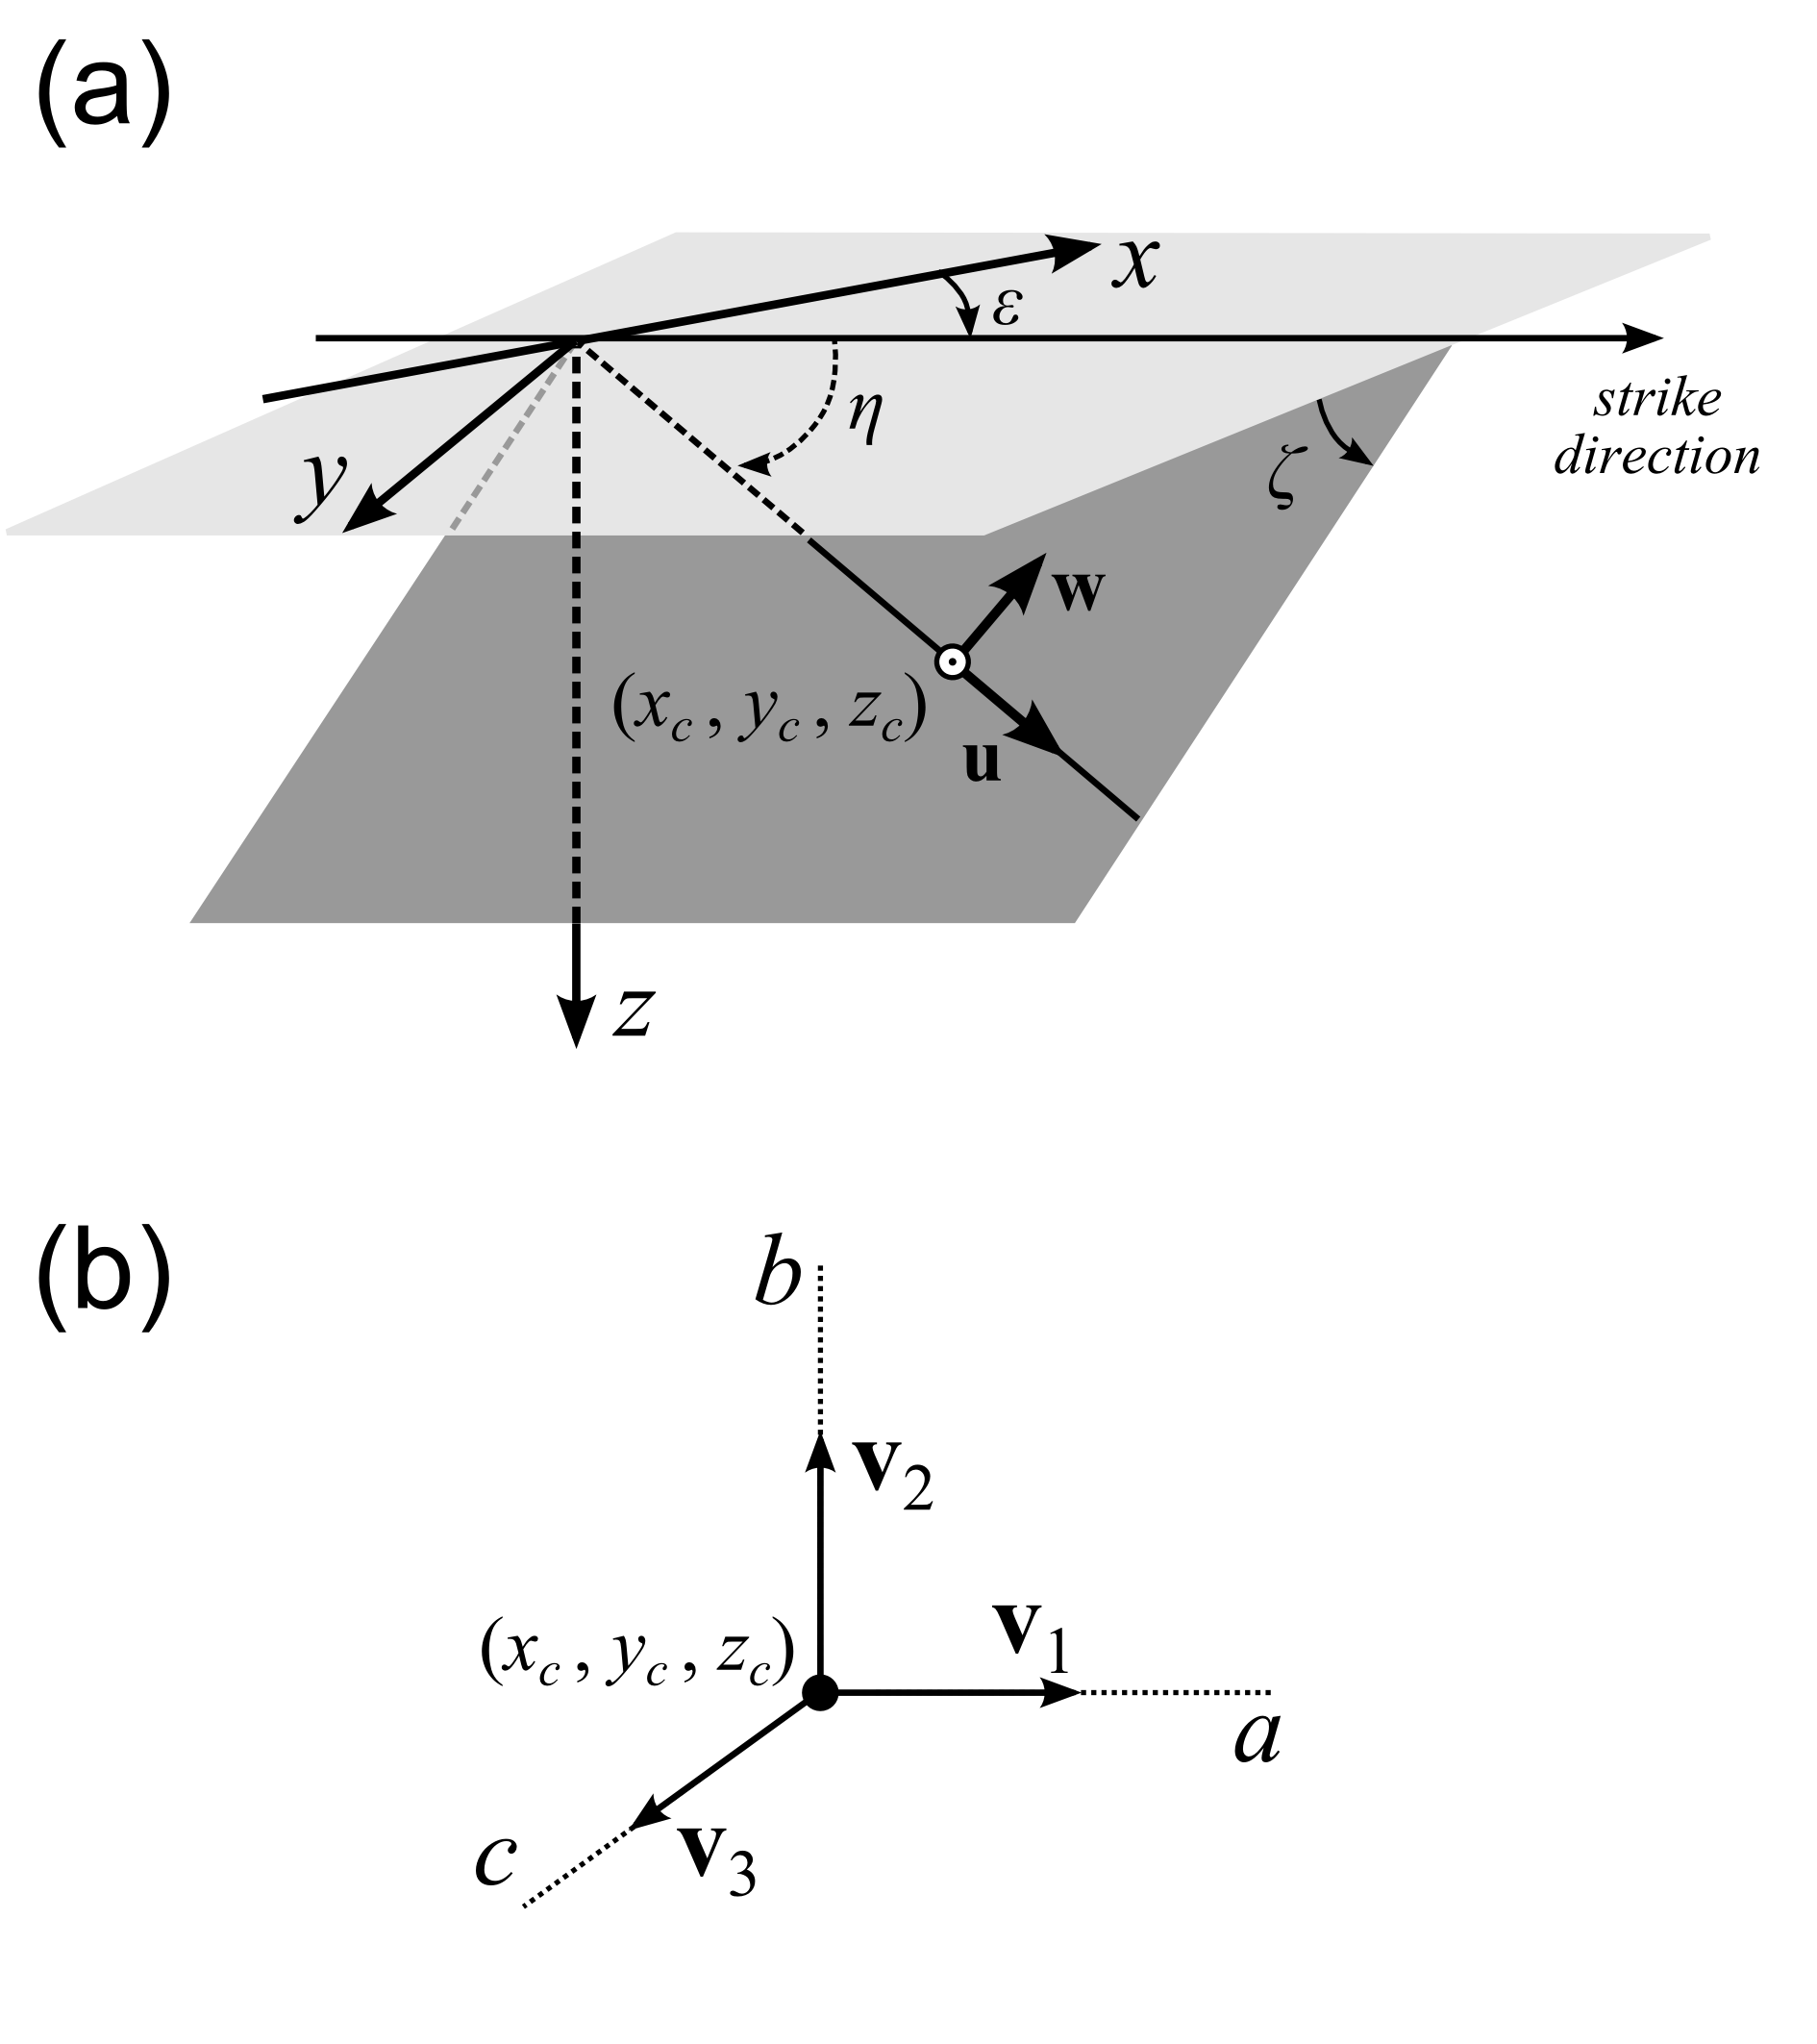
\includegraphics[width=8.3cm]{figures/structural_orientation_angles.png}
\caption{Schematic representation of the coordinate systems used to
represent an ellipsoidal body.
(a) Main coordinate system with axes $x$, $y$, and $z$ pointing to
North, East, ans down, respectively.
The dark gray plane contains the centre $(x_{c}, y_{c}, z_{c})$
(white circle) and two unit vectors, $\mathbf{u}$ and $\mathbf{w}$, defining two
semi-axes of the ellipsoidal body. For triaxial and prolate ellipsoids,
$\mathbf{u}$ and $\mathbf{w}$ define, respectively,
the semi-axes $a$ and $b$. For oblate ellipsoids, $\mathbf{u}$ and
$\mathbf{w}$ define the semi-axes $b$ and $c$, respectively.
The strike direction is defined by the intersection of the
dark gray plane and the horizontal plane (represented in light gray),
which contains the $x$ and $y$ axes. The angle $\varepsilon$
between the $x$-axis and the strike direction is called \textit{strike}.
The angle $\zeta$ between the horizontal plane and the dark gray plane
is called \textit{dip}. The angle $\eta$ between the strike direction
and the line containing the unit vector $\mathbf{u}$
is called \textit{rake}. The projection of this line on the
horizontal plane (not shown) is called \textit{dip direction}
\citep{pollard2005, allmendinger2012}. (b) Local coordinate system
with origin at the ellipsoid centre $(x_{c}, y_{c}, z_{c})$
(black dot) and axes defined by unit vectors $\mathbf{v}_{1}$,
$\mathbf{v}_{2}$, and $\mathbf{v}_{3}$. These unit vectors
define the semi-axes $a$, $b$, and $c$ of triaxial, prolate,
and oblate ellipsoids in the same way.
For triaxial and prolate ellipsoids,
the unit vectors $\mathbf{u}$ and $\mathbf{w}$ shown in (a) coincide
with $\mathbf{v}_{1}$ and $\mathbf{v}_{2}$, respectively. For
oblate ellipsoids, the unit vectors $\mathbf{u}$ and $\mathbf{w}$
shown in (a) coincide with $\mathbf{v}_{2}$ and $\mathbf{v}_{3}$,
respectively.}
\label{fig:orientation-angles}
\end{figure}

%f
\begin{figure}[t]
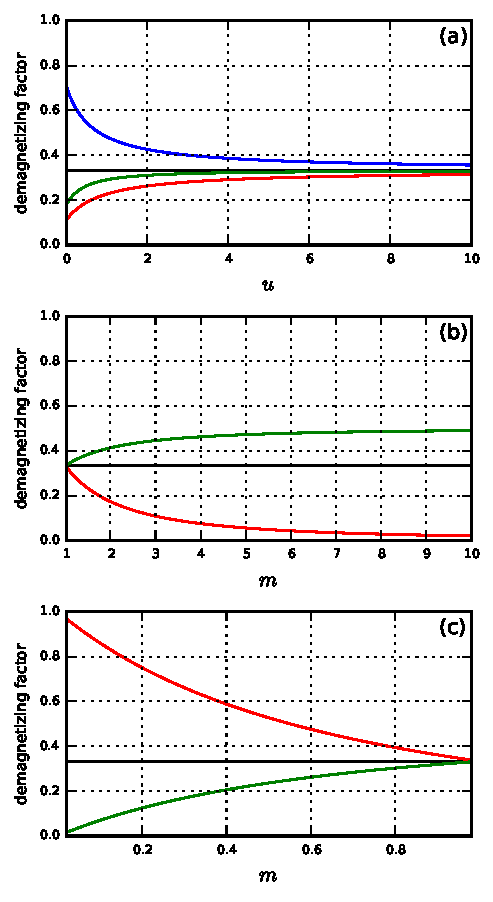
\includegraphics[width=8.3cm]{figures/demag_factors.pdf}
\caption{(a) Comparison between the demagnetizing factors
$\tilde{n}^{\dagger}_{11}$ (in red),
$\tilde{n}^{\dagger}_{22}$ (in green), and
$\tilde{n}^{\dagger}_{33}$ (in blue)
produced by 100 triaxial ellipsoids with semi-axes
$a = a_{0} + u \; b_{0}$, $b = b_{0} + u \; b_{0}$, and
$c = c_{0} + u \; b_{0}$, where $0 \leq u \leq 10$ and
$b_{0} = 700$ \unit{m}.
The demagnetizing factors were calculated
by using Eqs. \ref{eq:n-tilde-dagger-11-triaxial},
\ref{eq:n-tilde-dagger-22-triaxial}, and \ref{eq:n-tilde-dagger-33-triaxial}.
(b) Comparison between the demagnetizing factors
$\tilde{n}^{\dagger}_{11}$ (in red) and
$\tilde{n}^{\dagger}_{22}$ (in green)
produced by 100 prolate ellipsoids with semi-axes
$a = m \; b_{0}$ and $b = b_{0}$, where $1.02 \leq m \leq 10$ and
$b_{0} = 1000$ \unit{m}.
The demagnetizing factors were calculated
by using Eqs. \ref{eq:n-tilde-dagger-11-prolate} and
\ref{eq:n-tilde-dagger-22-prolate}.
(c) Comparison between the demagnetizing factors
$\tilde{n}^{\dagger}_{11}$ (in red) and
$\tilde{n}^{\dagger}_{22}$ (in green)
produced by 100 oblate ellipsoids with semi-axes
$a = m \; b_{0}$ and $b = b_{0}$, where $0.02 \leq m \leq 0.98$ and
$b_{0} = 1000$ \unit{m}.
The demagnetizing factors were calculated
by using Eqs. \ref{eq:n-tilde-dagger-11-oblate} and
\ref{eq:n-tilde-dagger-22-oblate}.
The horizontal black line represent the value $1/3$.}
\label{fig:demag-factors}
\end{figure}

%f
\begin{figure}[t]
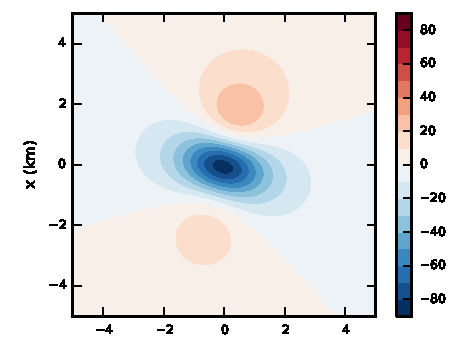
\includegraphics[width=8.3cm]{figures/confocal_ellipsoids_parallel_field.pdf}
\caption{Total-field anomaly (in \unit{nT}) produced by the 
synthetic bodies Ellipsoid 1 and Ellispoid 2, both
defined in Tab. \ref{tab:parameters-confocal-ellipsoids}.
The synthetic data produced by these confocal ellipsoids
were calculated on a regular grid of $200 \times 200$ points
at the constant vertical coordinate $z = 0$ \unit{m}.
These data were calculated with an uniform inducing field
parallel to the semi-axis $a$ of the confocal ellipsoids.}
\label{fig:tfa-confocal-ellipsoids-H0-parallel}
\end{figure}

%f
\begin{figure}[t]
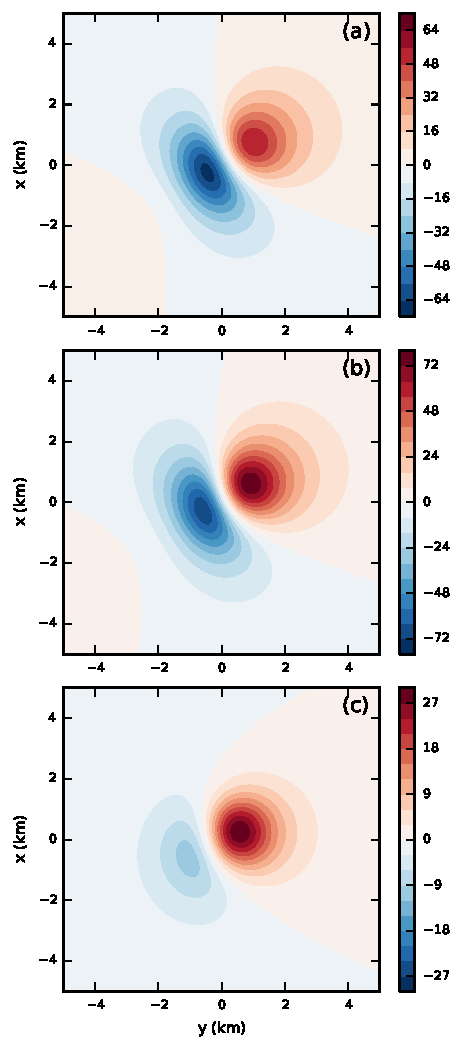
\includegraphics[width=8.3cm]{figures/confocal_ellipsoids_oblique_field.pdf}
\caption{Total-field anomalies (in \unit{nT}) produced by the (a) Ellipsoid 1
and (b) Ellipsoid 2, both defined in Tab. \ref{tab:parameters-confocal-ellipsoids}.
The synthetic data produced by these confocal ellipsoids
were calculated on a regular grid of $200 \times 200$ points
at the constant vertical coordinate $z = 0$ \unit{m}.
These data were calculated with an uniform inducing field
which is oblique to the semi-axes of the confocal ellipsoids.
(c) Difference between the total-field anomalies shown in
b and a.}
\label{fig:tfa-confocal-ellipsoids-H0-oblique}
\end{figure}

%f
\begin{figure}[t]
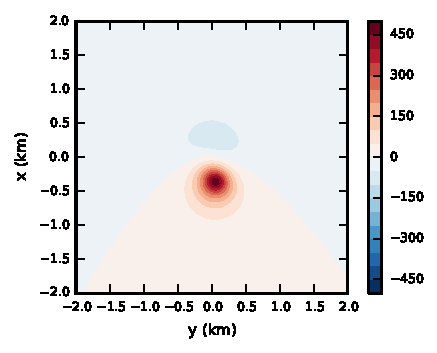
\includegraphics[width=8.3cm]{figures/total-field_anomaly.pdf}
\caption{Total-field anomaly (in \unit{nT}) produced by the synthetic orebody
defined in Tab. \ref{tab:parameters-warrego}. The synthetic data
are calculated on a regular grid of $100 \times 100$ points
at the constant vertical coordinate $z = 0$ \unit{m}.}
\label{fig:tfa-warrego}
\end{figure}

%f
\begin{figure}[t]
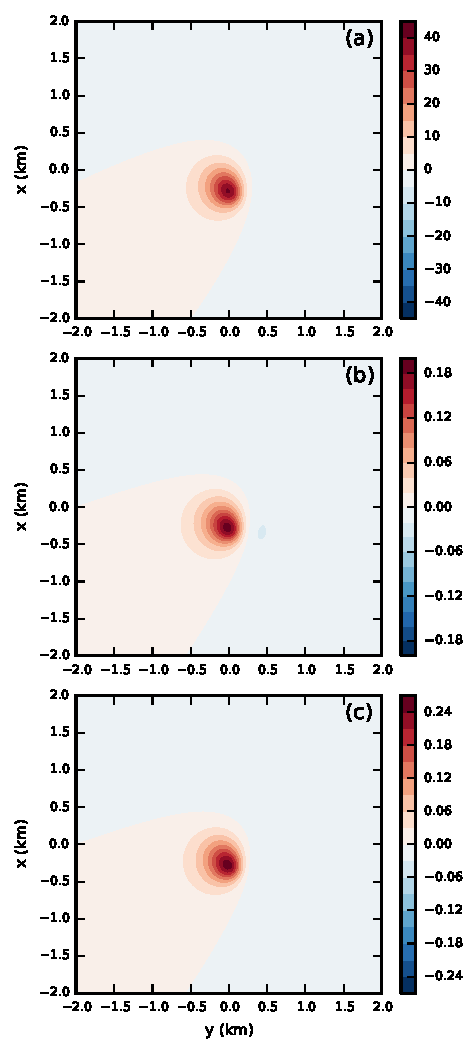
\includegraphics[width=8.3cm]{figures/field_differences.pdf}
\caption{Difference between the total-field
anomaly calculated with the approximated magnetization $\breve{\mathbf{M}}$
(Eq. \ref{eq:M-approx}) and with the
true magnetization $\mathbf{M}$
(Eqs. \ref{eq:M-K-isotropic} and \ref{eq:M-K-isotropic-inverse-Lambda}).
The total-field anomalies are in \unit{nT} and were
calculated with Eq. \ref{eq:delta-T-approx},
on a regular grid of $100 \times 100$ points,
at the constant vertical coordinate $z = 0$ \unit{m}.
The differences are produced by the synthetic orebody defined in
Tab. \ref{tab:parameters-warrego}, but with different
isotropic susceptibilities:
(a) the isotropic susceptibility defined in
Tab. \ref{tab:parameters-warrego},
(b) an isotropic susceptibility $\chi = 0.1$ \unit{SI}, and
(c) an isotropic susceptibility $\chi = 0.116$ \unit{SI}.
This last value was calculated
with Eq. \ref{eq:chi-max}, by using $\epsilon = 8 \%$.}
\label{fig:tfa-differences-warrego}
\end{figure}

%%% TWO-COLUMN FIGURES
%
%%f
%\begin{figure*}[t]
%\includegraphics[width=12cm]{FILE NAME}
%\caption{TEXT}
%\end{figure*}
%
%
%%% TABLES
%%%
%%% The different columns must be seperated with a & command and should
%%% end with \\ to identify the column brake.
%
%%% ONE-COLUMN TABLE
%
%%t
%\begin{table}[t]
%\caption{TEXT}
%\begin{tabular}{column = lcr}
%\tophline
%
%\middlehline
%
%\bottomhline
%\end{tabular}
%\belowtable{} % Table Footnotes
%\end{table}
%

\newpage

%t
\begin{table}[t]
\caption{Parameters defining two confocal ellipsoids.}
%\begin{tabular}{column = lcr}
\begin{tabular}{lccr}
\tophline
Parameter & Ellipsoid 1 & Ellipsoid 2 & Unit \\
\middlehline
Semi-axis $a$ & $900$ & $\approx 1676.31$ & \unit{m} \\
Semi-axis $b$ & $500$ & $1500$ & \unit{m} \\
Semi-axis $c$ & $100$ & $\approx 1417.74$ & \unit{m} \\
Coordinate of the centre $x_{c}$ & 0 & 0 & \unit{m} \\
Coordinate of the centre $y_{c}$ & 0 & 0 & \unit{m} \\
Coordinate of the centre $z_{c}$ & 1500 & 1500 & \unit{m} \\
Orientation angle $\varepsilon$ $^{\ast}$ & $45$ & $45$ & $^{\circ}$ \\
Orientation angle $\zeta$ $^{\ast}$ & $10$ & $10$ & $^{\circ}$ \\
Orientation angle $\eta$ $^{\ast}$ & $-30$ & $-30$ & $^{\circ}$ \\
Isotropic susceptibility $\chi$ & $1.2$ & $\approx 0.014$ & \unit{SI} \\
\bottomhline
\end{tabular}
\belowtable{$^{\ast}$ Defined in Fig. \ref{fig:orientation-angles}a} % Table Footnotes
\label{tab:parameters-confocal-ellipsoids}
\end{table}

%t
\begin{table}[t]
\caption{Parameters defining a synthetic orebody. This model is
based on the that presented by \citet{farrar1979} to simulate
the Warrego orebody, Tennant Creek field, Australia.}
%\begin{tabular}{column = lcr}
\begin{tabular}{lcr}
\tophline
Parameter & Value & Unit \\
\middlehline
Semi-axis $a$ & $490.7$ & \unit{m} \\
Semi-axis $b$ & $69.7$ & \unit{m} \\
Semi-axis $c$ & $30.0$ & \unit{m} \\
Coordinate of the centre $x_{c}$ & 0 & \unit{m} \\
Coordinate of the centre $y_{c}$ & 0 & \unit{m} \\
Coordinate of the centre $z_{c}$ & 500 & \unit{m} \\
Orientation angle $\varepsilon$ $^{\ast}$ & $-34.0$ & $^{\circ}$ \\
Orientation angle $\zeta$ $^{\ast}$ & $66.1$ & $^{\circ}$ \\
Orientation angle $\eta$ $^{\ast}$ & $45.0$ & $^{\circ}$ \\
Isotropic susceptibility $\chi$ & $1.69$ & \unit{SI} \\
$x$-component of the inducing field $\mathbf{B}_{0}$ $^{\dagger}$ & 32610 & \unit{nT} \\
$y$-component of the inducing field $\mathbf{B}_{0}$ $^{\dagger}$ & 0 & \unit{nT} \\
$z$-component of the inducing field $\mathbf{B}_{0}$ $^{\dagger}$ & 39450 & \unit{nT} \\
\bottomhline
\end{tabular}
\belowtable{$^{\ast}$ Defined in Fig. \ref{fig:orientation-angles}a \newline
$^{\dagger}$ Defined in Eq. \ref{eq:delta-T}} % Table Footnotes
\label{tab:parameters-warrego}
\end{table}

%%% TWO-COLUMN TABLE
%
%%t
%\begin{table*}[t]
%\caption{TEXT}
%\begin{tabular}{column = lcr}
%\tophline
%
%\middlehline
%
%\bottomhline
%\end{tabular}
%\belowtable{} % Table Footnotes
%\end{table*}
%
%
%%% NUMBERING OF FIGURES AND TABLES
%%%
%%% If figures and tables must be numbered 1a, 1b, etc. the following command
%%% should be inserted before the begin{} command.
%
%\addtocounter{figure}{-1}\renewcommand{\thefigure}{\arabic{figure}a}
%
%
%%% MATHEMATICAL EXPRESSIONS
%
%%% All papers typeset by Copernicus Publications follow the math typesetting regulations
%%% given by the IUPAC Green Book (IUPAC: Quantities, Units and Symbols in Physical Chemistry,
%%% 2nd Edn., Blackwell Science, available at: http://old.iupac.org/publications/books/gbook/green_book_2ed.pdf, 1993).
%%%
%%% Physical quantities/variables are typeset in italic font (t for time, T for Temperature)
%%% Indices which are not defined are typeset in italic font (x, y, z, a, b, c)
%%% Items/objects which are defined are typeset in roman font (Car A, Car B)
%%% Descriptions/specifications which are defined by itself are typeset in roman font (abs, rel, ref, tot, net, ice)
%%% Abbreviations from 2 letters are typeset in roman font (RH, LAI)
%%% Vectors are identified in bold italic font using \vec{x}
%%% Matrices are identified in bold roman font
%%% Multiplication signs are typeset using the LaTeX commands \times (for vector products, grids, and exponential notations) or \cdot
%%% The character * should not be applied as mutliplication sign
%
%
%%% EQUATIONS
%
%%% Single-row equation
%
%\begin{equation}
%
%\end{equation}
%
%%% Multiline equation
%
%\begin{align}
%& 3 + 5 = 8\\
%& 3 + 5 = 8\\
%& 3 + 5 = 8
%\end{align}
%
%
%%% MATRICES
%
%\begin{matrix}
%x & y & z\\
%x & y & z\\
%x & y & z\\
%\end{matrix}
%
%
%%% ALGORITHM
%
%\begin{algorithm}
%\caption{�}
%\label{a1}
%\begin{algorithmic}
%�
%\end{algorithmic}
%\end{algorithm}
%
%
%%% CHEMICAL FORMULAS AND REACTIONS
%
%%% For formulas embedded in the text, please use \chem{}
%
%%% The reaction environment creates labels including the letter R, i.e. (R1), (R2), etc.
%
%\begin{reaction}
%%% \rightarrow should be used for normal (one-way) chemical reactions
%%% \rightleftharpoons should be used for equilibria
%%% \leftrightarrow should be used for resonance structures
%\end{reaction}
%
%
%%% PHYSICAL UNITS
%%%
%%% Please use \unit{} and apply the exponential notation


\end{document}
